%% Преамбула TeX-файла

% 1. Стиль и язык
\documentclass[utf8x, 12pt]{G7-32} % Стиль (по умолчанию будет 14pt)

% Остальные стандартные настройки убраны в preamble-std.tex
\sloppy

% 1. Настройки стиля ГОСТ 7-32
% Для начала определяем, хотим мы или нет, чтобы рисунки и таблицы нумеровались в пределах раздела, или нам нужна сквозная нумерация.
% А не забыл ли автор букву 't' ?
\EqInChapter % формулы будут нумероваться в пределах раздела
\TableInChapter % таблицы будут нумероваться в пределах раздела
\PicInChapter % рисунки будут нумероваться в пределах раздела

% 2. Добавляем гипертекстовое оглавление в PDF
\usepackage[
bookmarks=true, colorlinks=true, unicode=true,
urlcolor=black,linkcolor=black, anchorcolor=black,
citecolor=black, menucolor=black, filecolor=black,
]{hyperref}

% 3. Изменение начертания шрифта --- после чего выглядит таймсоподобно.
% apt-get install scalable-cyrfonts-tex

\IfFileExists{cyrtimes.sty}
    {
        \usepackage{cyrtimes}
    }
    {
        % А если Times нету, то будет CM...
    }


% 4. Прочие полезные пакеты.
%\usepackage{underscore} % Ура! Теперь можно писать подчёркивание.
                        % И нельзя использовать подчёркивание в файлах.
                        % Выбирай, но осторожно.

\usepackage{graphicx}   % Пакет для включения рисунков

 % 5. Любимые команды
\newcommand{\Code}[1]{\textbf{#1}}

% 6. Поля
% С такими оно полями оно работает по-умолчанию:
% \RequirePackage[left=20mm,right=10mm,top=20mm,bottom=20mm,headsep=0pt]{geometry}
% Если вас тошнит от поля в 10мм --- увеличивайте до 20-ти, ну и про переплёт не забывайте:
\geometry{right=20mm}
\geometry{left=30mm}


% 7. Tikz
\usepackage{tikz}
\usetikzlibrary{arrows,positioning,shadows}

% 8 Листинги

\usepackage{listings}

% Значения по умолчанию
\lstset{
  inputencoding=utf8x,
  language=C,						% the language of the code
  basicstyle=\small\tt,				% the size of the fonts that are used for the code
  numbers=left,						% where to put the line-numbers
  numberstyle=\tiny\color{gray},	% the style that is used for the line-numbers
  stepnumber=1,						% the step between two line-numbers. If it's 1, each line 
									% will be numbered
  numbersep=5pt,					% how far the line-numbers are from the code
  backgroundcolor=\color{white},	% choose the background color. You must add \usepackage{color}
  showspaces=false,					% show spaces adding particular underscores
  showstringspaces=false,			% underline spaces within strings
  showtabs=false,					% show tabs within strings adding particular underscores
  frame=none,						% adds a frame around the code
  rulecolor=\color{black},			% if not set, the frame-color may be changed on line-breaks within not-black text (e.g. commens (green here))
  tabsize=3,						% sets default tabsize to 2 spaces
  captionpos=b,						% sets the caption-position to bottom
  breaklines=true,					% sets automatic line breaking
  breakatwhitespace=false,			% sets if automatic breaks should only happen at whitespace
  title=\lstname,					% show the filename of files included with \lstinputlisting;
									% also try caption instead of title
  keywordstyle=\color{black},		% keyword style
  commentstyle=\color{black},		% comment style
  stringstyle=\color{black},		% string literal style
  escapeinside={\%*}{*)},			% if you want to add LaTeX within your code
  morekeywords={*,...}				% if you want to add more keywords to the set
}

% Стиль для псевдокода: строчки обычно короткие, поэтому размер шрифта побольше
\lstdefinestyle{pseudocode}{
  basicstyle=\small,
  keywordstyle=\color{black}\bfseries\underbar,
  language=Pseudocode,
  numberstyle=\footnotesize,
  commentstyle=\footnotesize\it
}

% Стиль для обычного кода: маленький шрифт
\lstdefinestyle{realcode}{
  basicstyle=\scriptsize,
  numberstyle=\footnotesize
}

% Стиль для коротких кусков обычного кода: средний шрифт
\lstdefinestyle{simplecode}{
  basicstyle=\footnotesize,
  numberstyle=\footnotesize
}

% Стиль для BNF
\lstdefinestyle{grammar}{
  basicstyle=\footnotesize,
  numberstyle=\footnotesize,
  stringstyle=\bfseries\ttfamily,
  language=BNF
}

% Определим свой язык для написания псевдокодов на основе Python
\lstdefinelanguage[]{Pseudocode}[]{Python}{
  morekeywords={each,empty,wait,do},% ключевые слова добавлять сюда
  morecomment=[s]{\{}{\}},% комменты {а-ля Pascal} смотрятся нагляднее
  literate=% а сюда добавлять операторы, которые хотите отображать как мат. символы
    {->}{\ensuremath{$\rightarrow$}~}2%
    {<-}{\ensuremath{$\leftarrow$}~}2%
    {:=}{\ensuremath{$\leftarrow$}~}2%
    {<--}{\ensuremath{$\Longleftarrow$}~}2%
}[keywords,comments]

% Свой язык для задания грамматик в BNF
\lstdefinelanguage[]{BNF}[]{}{
  morekeywords={},
  morecomment=[s]{@}{@},
  morestring=[b]",%
  literate=%
    {->}{\ensuremath{$\rightarrow$}~}2%
    {*}{\ensuremath{$^*$}~}2%
    {+}{\ensuremath{$^+$}~}2%
    {|}{\ensuremath{$|$}~}2%
}[keywords,comments,strings]

% Подписи к листингам на русском языке.
\renewcommand*\thelstnumber{\oldstylenums{\the\value{lstnumber}}}
\renewcommand\lstlistingname{\cyr\CYRL\cyri\cyrs\cyrt\cyri\cyrn\cyrg}
\renewcommand\lstlistlistingname{\cyr\CYRL\cyri\cyrs\cyrt\cyri\cyrn\cyrg\cyri}

% Произвольная нумерация списков.
\usepackage{enumerate}

% PDF concatenation
\usepackage{pdfpages}

% Conditional compilation
\usepackage{ifthen}
\begin{document}
\frontmatter % выключает нумерацию ВСЕГО; здесь начинаются ненумерованные главы: реферат, введение, глоссарий, сокращения и прочее

\graphicspath{{../../inc/img/}}
\newcommand{\deft}[1]{{\bf\emph{#1}}}
\newtheorem{definition}{Определение}[section]
\newtheorem{theorem}{Теорема}[section]
\newcommand{\ntheorem}[2]{\begin{theorem} \deft{(#1).} #2 \end{theorem}}

% Команды \breakingbeforechapters и \nonbreakingbeforechapters
% управляют разрывом страницы перед главами.
% По-умолчанию страница разрывается.

% \nobreakingbeforechapters
% \breakingbeforechapters

% Title page
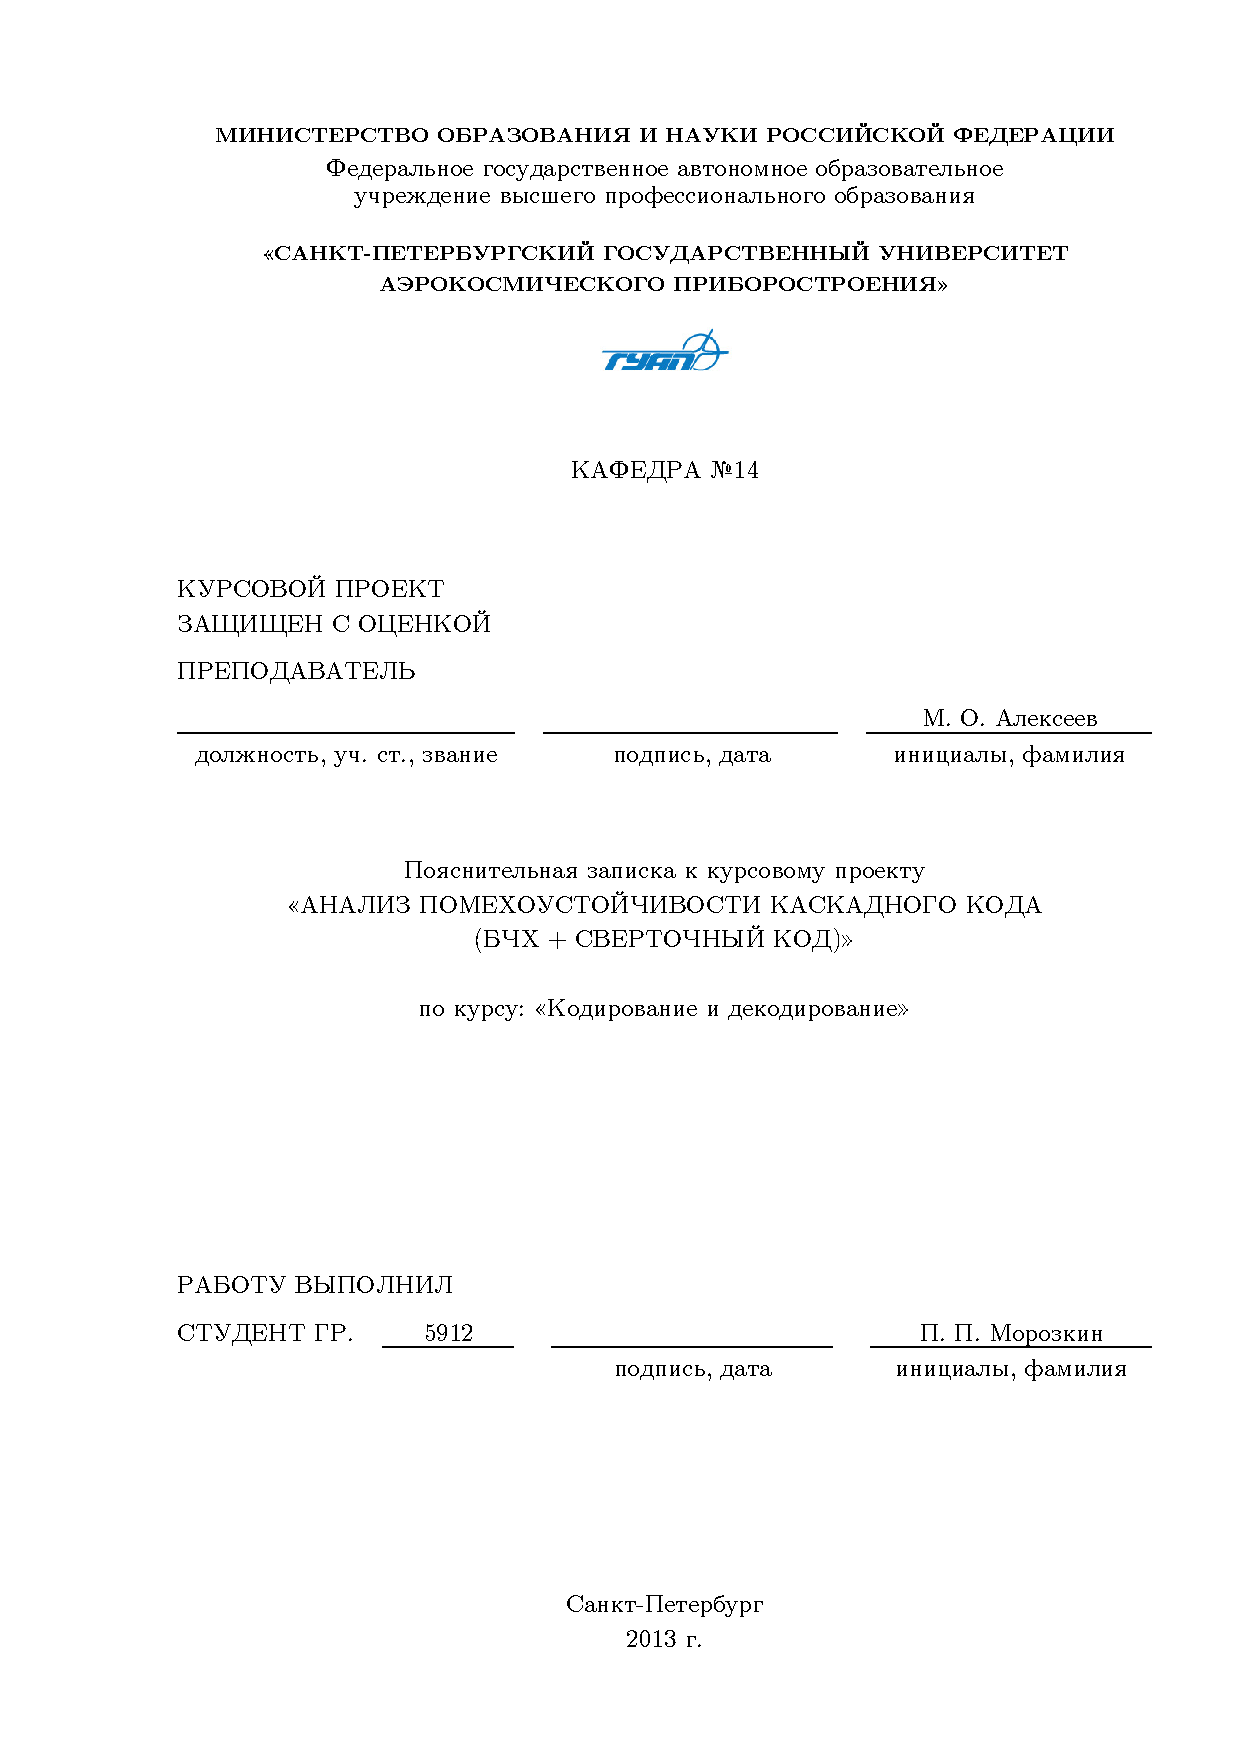
\includepdf[pages=-]{../../inc/img/tit/tit.pdf}

% Также можно использовать \Referat, как в оригинале
%\begin{abstract}
%Благодарности
%\end{abstract}

%%% Local Variables: 
%%% mode: latex
%%% TeX-master: "rpz"
%%% End: 

\tableofcontents
% Включает нумерацию глав и секций в документе ниже
\mainmatter
\Abbreviations %% Список обозначений и сокращений в тексте
\begin{description}

\item[БЧХ-код] Код Боуза — Чоудхури — Хоквингема

\end{description}

%%% Local Variables:
%%% mode: latex
%%% TeX-master: "rpz"
%%% End:

\Introduction

В настоящий момент потребность в надежной передаче данных между устройствами остается актуальной. Это 
связано с тем, что в любом реальном физическом канале связи присутствуют посторонние шумы, искажающие 
поступающие данные. Для устранения искажений и получения оригинальной информации в настоящее время 
широко используется помехоустойчивое кодирование информации. Исходный поток данных разбивается на 
порции данных, которые кодируются помехоустойчивым кодом и передаются в закодированном виде в канал 
связи. После принятия искаженных данных из канала выполняется процесс декодирования полученной 
информации. В случае обнаружения ошибок используются алгоритмы, позволяющие восстановить оригинальную 
информацию. При использовании кодирования к исходным данным добавляется избыточная информация, которая 
позволяет на этапе декодирования определить наличие ошибок и выполнить их устранение.

Пионером теории кодирования приято считать Клода Шеннона, опубликовавшего в 1948 году статью, в которой 
он определил понятие \textit{пропускной способности} канала. Было показано, что для каждого канала 
пропускная способность определяется числом $С$ и измеряется в битах в секунду. Затем было показано, что 
если скорость передачи данных $R$ (бит/сек) меньше, чем пропускная способность канала, то с 
использованием помехоустойчивых кодов можно добиться сколь угодно малой вероятности ошибки на выходе. В 
дальнейшем многие исследователи приложили свои усилия для отыскания классов кодов, которые позволяют 
получить малую вероятность ошибки. В частности, одно из направлений было посвящено изучению \textit{
блоковых кодов}. 

Первые блоковые коды были описаны Хеммингом в 1950 году. Он показал, что найденный им класс кодов 
позволяет строить коды, способные исправлять одиночные ошибки. Данное открытие стало прорывом в теории 
кодирования, и многие исследователи, воодушевленные работой Хемминга, продолжили поиски лучшего класса 
кодов. Однако, на протяжении десяти лет такой класс кодов получить не удалось. Но в 1960 году Боуз, 
Чоудхори и Хоквингем нашли класс кодов, позволяющих исправлять кратные ошибки. Полученные ими коды 
подучили название БЧХ-коды.

Другой класс кодов, позволяющий строить коды и кодировать ими информацию, получил название \textit{
сверточных кодов}. Развитие сверточных кодов заметно отличалось от развития теории блоковых кодов. 
Разницу можно почуствовать даже если сравнить подходы для нахождения хороших классов кодов. Так, при 
построении блоковых кодов и создании эффективных алгоритмов декодирования широко используются \textit{
алгебраические методы}. Со сверточными кодами ситуация иная. Например, хорошие сверточные коды были 
найдены с использованием вычислительной техники. Для этого выполнялся анализ большого числа кодов, а 
затем выбирались коды с лучшими характеристиками.

Другим отличительным свойством сверточных кодов является отсутствие методов декодирования, аналогичных 
алгебраическим методам исправления кратных ошибок. Наиболее используемым методом декодирования 
сверточных кодов является \textit{метод максимального правдоподобия}, на основе которого функционирует 
\textit{алгоритм Витерби}. Сверточное кодирование и декодирование с использованием алгоритма Витерби 
стало широко применяться на практике. Например, указанное кодирование применяется при передаче денных в 
космическом пространстве и при передаче денных из космического пространства на Землю и обратно. 
Причина, по которой данное кодирование столь распространено, состоит в относительной простоте 
реализации и в достижении выигрыша при декодировании.

Для улучшения характеристик системы передачи информации было предложено использовать \textit{каскадные 
коды}. В этом случае исходных поток данных после его разбиения на порции данных кодируется одним их 
блоковых кодов. Широко используемым кодом для данной цели является БЧХ-код. Далее полученное кодовое 
слово БЧХ-кода кодируется сверточным кодом. Полученное слово сверточного кода отправляется в канал. 
Таким образом два кодера работают в каскаде, откуда и произошло характерное название данного класса 
кодов. При декодировании каскадного кода выполняется ряд обратных кодированию процедур. Так, на первом 
этапе с использованием алгоритма Витерби происходит декодирование данных, поступивших из канала. В 
результате декодирования имеем кодовое слово БЧХ-кода, которое дополнительно декодируется БЧХ-
декодером. Особая эффективность такого способа кодирования состоит в том, что характерные свойства как 
БЧХ-кодов, так и сверточных кодов (и алгоритма Витерби) используются совместно, что позволяет достигать 
более высоких показателей, таких как вероятность ошибки на бит. Недостатком такого подхода является, 
пожалуй, относительная низкая скорость кода.
\chapter{Структура системы передачи информации}

Система передачи информации показана на Рис.~\ref{img_01}. Она состоит из источника информации, генерирующего исходный 
поток данных. Источник информации передает данные в кодер источника информации, который предназначен для устранения 
естественной избыточности генерируемой информации. Кодированные данные затем поступают в кодер канала. Данный 
компонент предназначен для кодирования данных помехоустойчивым кодом для возможности обнаружения ошибок на удаленной 
стороне и восстановления исходных данных.

\begin{figure}[htbp]
\begin{center}
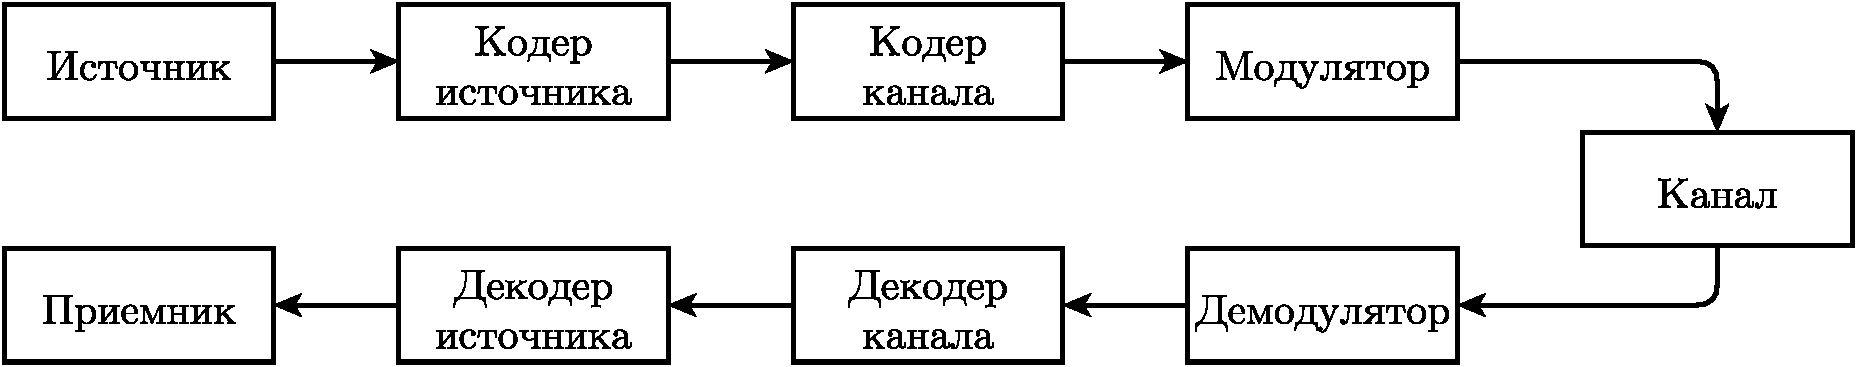
\includegraphics[scale=0.45]{chapter_1/img_01.pdf}
\end{center}
\caption{Структура системы передачи информации}
\label{img_01}
\end{figure}

Таким образом, кодированные данные поступают в модулятор, который предназначен для генерации по цифровым данным реальных физических сигналов и их передачу в канал. Причем в данной ситуации каналом может являться как телефонный кабель, оптическое волокно, воздушная среда, так и система хранения информации, например, жесткий диск, магнитный диск или флеш- накопитель. По сути, все эти устройства реализуют канал связи, который в общих чертах можно охарактеризовать как компонент, позволяющий передавать данные и обладающий тем свойством, что при передаче данных могут возникать ошибки. Их появление объясняется природой канала и не может быть определено заранее. После передачи данных каналом и получения данных на удаленной стороне начинается обратный процесс, нацеленный на восстановление переданных данных. Вначале данные из канала демодулируются демодулятором, который генерирует кодовые слова выбранного кода. Данные слова декодируются декодером канала. В случае обнаружения декодером ошибок при передаче данных, выполняется процесс устранения данных ошибок с целью получить исходные денные. В результате декодирования данные поступают в декодер источника. На этом этапе выполняется декодирование данных, изначально сгенерированных источником, добавляется избыточная информация. Полученные денные отправляются приемнику информации.
\chapter{Теретические основы кодов, контролирующих ошибки}

В данном разделе приводятся сведения о кодах, контролирующих ошибки, необходимые для дальнейшего изложения
материала.

%%%%%%%%%%%%%%%%%%%%%%%%%%%%%%%%%%%%%%%%%%%%%%%%%%%%%%%%%%%%%%%%%%%%%%%%%%%%%%%%%%%%%%%%%%%
%%%%%%%%%%%%%%%%%%%%%%%%%%%%%%%%%%%%%%%%%%%%%%%%%%%%%%%%%%%%%%%%%%%%%%%%%%%%%%%%%%%%%%%%%%%
%%%%%%%%%%%%%%%%%%%%%%%%%%%%%%%%%%%%%%%%%%%%%%%%%%%%%%%%%%%%%%%%%%%%%%%%%%%%%%%%%%%%%%%%%%%
\section{Блоковые коды}
\begin{definition} 
\deft{Блоковый код} мощности $M$ над алфавитом из $q$ символов --- это множество из $M$ $q$-ичных последовательностей длины $n$, называемых \emph{кодовыми словами}. 
\end{definition}

При $q=2$ символы называются \deft{битами}, а код --- \deft{двоичным}. Как правило, $M=q^k$ для некоторого $k$. Такой код носит название \emph{$(n,k)$-код}. Каждой последовательности из $k$ $q$-ичных символов можно сопоставить последовательность из $n$ $q$-ичных символов, которая и является кодовым словом. Блоковый код задает $n$-символьное кодовое слово, которое включает $k$ информационных символов.

\begin{definition}
\deft{Скорость} блокового кода --- величина $R=k/n$.
\end{definition}

Основные параметры блокового кода:
\begin{enumerate}
\item длина блока $n$
\item информационная длина $k$
\item минимальное расстоянию $d^*$
\end{enumerate}

Минимальное расстояние является мерой различия двух наиболее похожих кодовых слов.

\begin{definition}
\deft{Расстояние по Хеммингу} между двумя $q$-ичными последовательностями $x$ и $y$ длины $n$ --- число позиций, в которых данные последовательности отличаются. Обозначение: $d(x, y)$.
\end{definition}

Пример расстояния, $d(01011, 00111)=2$.

\begin{definition} 
Пусть $\mathfrak{C}=\{c_i, i=0, \ldots, M - 1\}$~---~код. Тогда \deft{минимальное 
расстояние} кода $\mathfrak{C}$ равно наименьшему из всех расстояний по Хеммингу между различными парами 
кодовых слов, т.е. 
$$ d^*  = \mathop {\mathop {\min }\limits_{c_i ,\,c_j  \in \mathfrak{C}} }\limits_{i \ne j}
\left( {c_i ,\;c_j } \right) $$ 
\end{definition}

\begin{definition} 
$(n, k)$-код с минимальным расстоянием $d^*$ называется $(n, k, d^*)$-кодом.
\end{definition}

В случае возникновения в канале $t$ ошибок при передаче кодового слова результат декодирования зависит
от расстояния от принятого слова до каждого другого слова. Так, в случае, если расстояние от принятого
слова до каждого другого кодового слова превосходит $t$, то ошибки будут исправлены, а ближайшее
к принятому кодовое слово будет принято в качестве действительно переданного. Данное утверждение
выполняется только в случае $$d^* \geq 2t+1.$$

%%%%%%%%%%%%%%%%%%%%%%%%%%%%%%%%%%%%%%%%%%%%%%%%%%%%%%%%%%%%%%%%%%%%%%%%%%%%%%%%%%%%%%%%%%%
%%%%%%%%%%%%%%%%%%%%%%%%%%%%%%%%%%%%%%%%%%%%%%%%%%%%%%%%%%%%%%%%%%%%%%%%%%%%%%%%%%%%%%%%%%%
%%%%%%%%%%%%%%%%%%%%%%%%%%%%%%%%%%%%%%%%%%%%%%%%%%%%%%%%%%%%%%%%%%%%%%%%%%%%%%%%%%%%%%%%%%%
\subsection{Линейные блоковые коды}

Большинство известных хороших кодов принадлежат классу \deft{линейных кодов}.

\begin{definition} 
\deft{Линейный код} --- подпространство в векторном пространстве $GF^n(q)$.
\end{definition}

Таким образом, линейный код есть непустое множество $n$-последовательностей над
полем Галуа $GF(q)$. Данные последовательности называемых кодовыми словами. Особенностью множества
является то, что сумма двух кодовых слов является кодовым словом, а произведение любого кодового слова на элемент поля также является кодовым словом.

\begin{definition}
\deft{Систематический код} --- код, у которого всякое кодовое слово начинается с информационных символов. Оставшиеся символы называются \deft{проверочными символами}.
\end{definition}

\begin{definition} \deft{Вес Хемминга $\omega(с)$} кодового слова $c$ --- число ненулевых компонент.
\deft{Минимальный вес кода $\omega^*$} --- минимальный вес ненулевого кодового слова.
\end{definition}

\begin{theorem} 
Для линейного кода минимальное расстояние $d^*$ равно минимальному весу $\omega^*$.
\end{theorem}

\begin{theorem} 
Минимальное расстояние любого линейного $(n, k)$-кода удовлетворяет неравенству $$d^* \leq 1+n-k.$$
\end{theorem}

\begin{definition}
Любой $(n, k)$-код с минимальным расстоянием, которое удовлетворяет равенству $$d^*=1+n-k$$ называется
\deft{кодом с максимальным расстоянием}.
\end{definition}

Согласно Границе Синглтона для исправления $t$ ошибок код должен иметь не менее $2t$ проверочных
символов (2 проверочных символа на ошибку). Коды с максимальным расстоянием имеют точно $2t$
проверочных символов.

%%%%%%%%%%%%%%%%%%%%%%%%%%%%%%%%%%%%%%%%%%%%%%%%%%%%%%%%%%%%%%%%%%%%%%%%%%%%%%%%%%%%%%%%%%%
%%%%%%%%%%%%%%%%%%%%%%%%%%%%%%%%%%%%%%%%%%%%%%%%%%%%%%%%%%%%%%%%%%%%%%%%%%%%%%%%%%%%%%%%%%%
%%%%%%%%%%%%%%%%%%%%%%%%%%%%%%%%%%%%%%%%%%%%%%%%%%%%%%%%%%%%%%%%%%%%%%%%%%%%%%%%%%%%%%%%%%%
\subsection{Циклические коды}
Циклические коды составляют относительно большую группу наиболее широко используемых на 
практике линейных систематических кодов. Их основное свойство, давшее им название, 
заключается в том, что каждый вектор, получаемый из исходного кодового вектора путем 
циклической перестановки его символов, также является разрешенным кодовым вектором.
В качестве математического аппарата для построения данных кодов используется теория полей Галуа.

Операции кодирования и декодирования циклических кодов сводятся к известным процедурам 
умножения и деления полиномов. Для двоичных кодов эти операции легко реализуются 
технически с помощью линейных переключательных схем (ЛПС), при этом получаются 
относительно простые схемы кодеков, в чем состоит одно из практических достоинств циклических кодов.

\begin{definition}
Линейный $(n, k)$-код $\mathfrak{C}$ называется \deft{циклическим}, если
из того, что слово $c=(c_0, c_1, \ldots, c_{n-1})$ принадлежит коду $\mathfrak{C}$,
следует, что слово $c^\prime=(c_{n-1}, c_0, c_1, \ldots, c_{n-2})$ также принадлежит
коду $\mathfrak{C}$.
\end{definition}

Кодовое слово $c^\prime$ получается циклическим сдвигом всех компонент слова $c$ вправо
на одну позицию. Каждый линейный код над $GF(q)$ длины $n$ представляет собой
подпространство пространства $GF^n(q)$, а циклический код является частным случаем
подпространства, так как обладает дополнительным свойством цикличности.

Каждый вектор из $GF^n(q)$ можно представить многочленом от $x$ степени не выше $n-1$. Компоненты вектора 
отождествляются с коэффициентами многочлена. Множество многочленов обладает структурой векторного 
пространства, идентичной структуре пространства $GF^n(q)$. Это же множество многочленов обладает структурой 
кольца $GF(q)[x]/(x^n-1)$. Как в кольце, в этом множестве определено умножение $$p_1(x)\cdot p_2(x)=R_{x^n-1} 
\left[{p_1(x)p_2(x)}\right]$$ где $R_{h(x)}\left[{f(x)g(x)}\right]$~---~есть остаток от деления на многочлен $
 h(x)$ произведения многочленов $f(x)$ и $g(x)$. Заметим, что в приведенное равенство входят произведения 
двух видов. Произведение в левой части является произведением в кольце $GF(q)[x]/(x^n-1)$, определенным через 
произведения к кольце $GF(q)[x]$ в правой части. Циклический сдвиг может быть записан через умножение в этом 
кольце: $$x\cdot p(x)=R_{x^n-1}[xp(x)].$$

Итак, если кодовые слова некоторого кода задаются в виде многочленов, то код является подмножеством
кольца $GF(q)[x]/(x^n-1)$. Такой код является циклическим, если вместе с каждым кодовым словом $c(x)$
он содержит кодовый многочлен $x\cdot c(x)$.

\begin{definition}
\deft{Порождающий многочленом} кода $\mathfrak{C}$ --- единственный приведенный ненулевой многочлен наименьшей степени в коде $\mathfrak{C}$. Обозначение: $g(x)$.
\end{definition}

\begin{theorem} 
Циклический $(n, k)$-код состоит из всех произведений порождающего многочлена $g(x)$ степени $n-k$ на многочлены степени не выше $k-1$.
\end{theorem}

\begin{theorem}
\label{th5.2.3} Циклический код длины $n$ с порождающим многочленом $g(x)$ существует тогда
и только тогда, когда $g(x)$ делит $x^n-1$.
\end{theorem}

Согласно теореме \ref{th5.2.3}, для порождающего многочлена $g(x)$ любого циклического кода выполняется 
равенство $$x^n-1=g(x)h(x)$$ при некотором многочлене $h(x)$. Многочлен $h(x)$ называется \deft{проверочным 
многочленом}. Каждое кодовое слово $c(x)$ удовлетворяет равенству $$R_{x^n-1}[h(x)c(x)]=0.$$

Пусть $c(x)$ обозначает переданное кодовое слово. Это значит что символами переданного слова были 
коэффициенты многочлена $c(x)$. Пусть многочлен $v(x)$ обозначает принятое слово, и пусть $e(x)=v(x)-c(x)$. 
Многочлен $e(x)$ называется \deft{многочленом ошибок}. Ненулевые коэффициенты этого многочлена стоят в тех 
позициях, где в канале произошли ошибки.

Представим информационную последовательность в виде многочлена $i(x)$ степени не выше $k-1$. Множество 
информационных многочленов можно отобразить в кодовые многочлены многими способами. Одним простым правилом 
является $$c(x)=i(x)g(x).$$

Такой кодер является несистематическим, так как по многочлену $c(x)$ нельзя сразу установить $i(x)$. 
Систематическое правило кодирования имеет следующий вид: $$c(x)=x^{n-k}i(x)+t(x),$$ где $t(x)=-R_{g(x)}\left[x
^{n-k}i(x)\right]$.

И систематическое, и несистематическое правила кодирования дают одно и тоже множество кодовых слов, но 
соответствия между $i(x)$ и $c(x)$ различны.

\begin{definition}
\deft{Синдромный многочлен} $s(x)$ --- остаток от деления многочлена $v(x)$ на $g(x)$: $$s(x)=R_{g(x)}[v(x)]=R
_{g(x)}[c(x) + e(x)]=R_{g(x)}[e(x)].$$
\end{definition}

%%%%%%%%%%%%%%%%%%%%%%%%%%%%%%%%%%%%%%%%%%%%%%%%%%%%%%%%%%%%%%%%%%%%%%%%%%%%%%%%%%%%%%%%%%%
%%%%%%%%%%%%%%%%%%%%%%%%%%%%%%%%%%%%%%%%%%%%%%%%%%%%%%%%%%%%%%%%%%%%%%%%%%%%%%%%%%%%%%%%%%%
%%%%%%%%%%%%%%%%%%%%%%%%%%%%%%%%%%%%%%%%%%%%%%%%%%%%%%%%%%%%%%%%%%%%%%%%%%%%%%%%%%%%%%%%%%%
\section{БЧХ-коды}
Коды Боуза-Чоудхури-Хоквингема (БЧХ) составляют один из больших классов линейных кодов, исправляющих ошибки. 
Причем метод построения этих кодов задан явно. Интерес к кодам БЧХ определяется тем, что они позволяют 
исправлять любое наперед заданное число ошибок и для них существуют эффективные алгоритмы кодирования и 
декодирования.

Порождающий многочлен циклического кода можно представить в виде
$$g(x)=НОК\left[f_1(x), f_2(x), \ldots, f_r(x)\right],$$ где $f_i(x), i=1, \ldots, r$~---~минимальные
многочлены корней $g(x)$.

Пусть элементы $GF(q^m)$ $\gamma_1, \gamma_2, \ldots, \gamma_r$~---~корни порождающего многочлена
$g(x)$. Тогда $$v(\gamma_i)=c(\gamma_i)+e(\gamma_i)=e(\gamma_i)=\sum\limits_{j = 0}^{n - 1} {e_j \gamma _i^j }.$$

В результате получаем $r$ уравнений, содержащих только величины, определяемые ошибками и не зависящие от 
кодового слова. Если эти уравнения можно разрешить относительно $e_j$, то мы сможем определить многочлен 
ошибок. Нужно выбрать $\gamma_i$ таким образом, чтобы система $r$ уравнений могла быть решена относительно $e_
i$ каждый раз, когда не более $t$ неизвестных отличны от нуля.

Для произвольного циклического кода с порождающим многочленом $g(x)$, имеющим корни $\gamma_1, \ldots, \gamma_
r$, определим компоненты синдрома $$S_j=v(\gamma_j), j=1, \ldots, r.$$

Эти элементы поля отличны от синдромного многочлена $s(x)$, но содержат эквивалентную информацию. Мы хотим 
подобрать $\gamma_1, \ldots, \gamma_r$ так, чтобы по $S_1, \ldots, S_r$ можно было найти $t$ ошибок. В 
качестве таких $\gamma_i$ можно взять степени $\{\alpha, \alpha^2, \ldots, \alpha^{2t}\}$ примитивного 
элемента $\alpha$ поля $GF(q^m)$.

\begin{definition} 
Пусть заданы $q$ и $m$, и пусть $\beta$~---~любой элемент поля $GF(q^m)$ порядка $n$. Тогда для любого 
положительного целого числа $t$ % и любого целого числа $j_0$ соответствующий \deft{код БЧХ} является 
циклическим кодом длины $n$ с порождающим многочленом $$g(x)=НОК\left(f_{1}\left(x\right), \ldots, 
f_{2t}\left(x\right)\right),$$ где $f_j(x)$~---~минимальный многочлен элемента $\beta^j$.
\end{definition}

%Часто выбирают $j_0=1$, что, как правило, приводит к многочлену $g(x)$ с наименьшей степенью.

\begin{definition} 
\deft{Примитивный} БЧХ-код --- код длины $q^m-1$.
\end{definition}

Для того, чтобы построить порождающий многочлен примитивного БЧХ-кода нужно:
\begin{enumerate}
  \item Задать длину кода $n=q^m-1$ и число $t$ ошибок, которые необходимо исправлять.
  \item Найти неприводимый многочлен степени $m$ и построить поле $GF(q^m)$.
  \item Найти примитивный элемент $\alpha$ в поле $GF(q^m)$.
  \item Найти минимальные многочлены $f_i(x)$ для $\alpha^i, i=1, \ldots, 2t$ над $GF(q)$.
  \item Взять в качестве $g(x)=НОК\left({f_1(x), f_2(x), \ldots, f_{2t}(x)}\right).$
\end{enumerate}

%%%%%%%%%%%%%%%%%%%%%%%%%%%%%%%%%%%%%%%%%%%%%%%%%%%%%%%%%%%%%%%%%%%%%%%%%%%%%%%%%%%%%%%%%%%
%%%%%%%%%%%%%%%%%%%%%%%%%%%%%%%%%%%%%%%%%%%%%%%%%%%%%%%%%%%%%%%%%%%%%%%%%%%%%%%%%%%%%%%%%%%
%%%%%%%%%%%%%%%%%%%%%%%%%%%%%%%%%%%%%%%%%%%%%%%%%%%%%%%%%%%%%%%%%%%%%%%%%%%%%%%%%%%%%%%%%%%
\subsection{Поиск порождающего многочлена}
Для того, чтобы найти порождающий многочлен БЧХ, надо выполнить следующие шаги:
\begin{enumerate}
  \item Выбрать основание --- простое число $p$.
  \item Выбрать число членов поля $q=pk$, над которыми будет построен код БЧХ, где $k$ --- натуральное число.
  \item Определить длину кода $n$, дина кода $n$ определяется из формулы $n=\frac{q^m-1}{s}$, где $m$, $s$ ---
 натуральные числа.
  \item Задать желаемое минимальное расстояние для кода $d$, значение минимального расстояния кода $d$ должно 
быть меньше длины кода $n$.
  \item Построить поле $GF(q)$.
  \item Построить поле $GF(q^m)$, где $m$ --- параметр кода БЧХ.
  \item Найти примитивный элемент $\lambda$ поля $GF(q^m)$.
  \item Найти степень примитивного элемента $\beta=\lambda~s$, где $s$ --- параметр кода БЧХ.
  \item Найти $d-1$ последовательные степени $\beta: \beta^l, \beta^{l+1}, \beta^{l+2}, ... \beta^{l+d-2}$, 
где $l$ --- произвольное натуральное число.
  \item Найти нормированный многочлен $g(x)$ минимальной степени над полем $GF(q)$, корнями которого являются 
все $d–1$ подряд идущих степеней $\beta^l, \beta^{l+1}, \beta^{l+2}, ... \beta^{l+d-2}$.
  \item Этот многочлен $g(x)$ и является порождающим для БЧХ-кода с заданными выше параметрами.
\end{enumerate}

%%%%%%%%%%%%%%%%%%%%%%%%%%%%%%%%%%%%%%%%%%%%%%%%%%%%%%%%%%%%%%%%%%%%%%%%%%%%%%%%%%%%%%%%%%%
%%%%%%%%%%%%%%%%%%%%%%%%%%%%%%%%%%%%%%%%%%%%%%%%%%%%%%%%%%%%%%%%%%%%%%%%%%%%%%%%%%%%%%%%%%%
%%%%%%%%%%%%%%%%%%%%%%%%%%%%%%%%%%%%%%%%%%%%%%%%%%%%%%%%%%%%%%%%%%%%%%%%%%%%%%%%%%%%%%%%%%%
\subsection{Выбор параметров кода}
Параметры кода БЧХ выбираются исходя из требований задачи, в которой код будет применен. Ниже будет 
использоваться $p=2$ и $k=1$. Последнее обусловлено тем, что в основном коды БЧХ применяют в вычислительных 
устройствах, которые используют двоичное представление чисел и, следовательно, удобнее использовать двоичные 
коды БЧХ.

%%%%%%%%%%%%%%%%%%%%%%%%%%%%%%%%%%%%%%%%%%%%%%%%%%%%%%%%%%%%%%%%%%%%%%%%%%%%%%%%%%%%%%%%%%%
%%%%%%%%%%%%%%%%%%%%%%%%%%%%%%%%%%%%%%%%%%%%%%%%%%%%%%%%%%%%%%%%%%%%%%%%%%%%%%%%%%%%%%%%%%%
%%%%%%%%%%%%%%%%%%%%%%%%%%%%%%%%%%%%%%%%%%%%%%%%%%%%%%%%%%%%%%%%%%%%%%%%%%%%%%%%%%%%%%%%%%%
\subsection{Построение конечного поля}
Существует два варианта построения поля, в зависимости от количества элементов.
\begin{enumerate}
  \item Поле содержит $p$ элементов, где $p$ --- простое. В данном случае полем является кольцо вычетов по 
модулю $p$.
  \item Поле содержит $q=pk$ элементов, где $p$ --- простое, $k$ --- натуральное числа. Для построения поля 
из $q=pk$ элементов достаточно отыскать многочлен $f(x)$ степени $k$, неприводимый над полем $GF(p)$.
\end{enumerate}
В случае кодов БЧХ оба поля, используемые в построении, являются полями $GF(q)$ и $GF(q^m)$, т.е. для их 
построения необходимо отыскание двух неприводимых многочленов --- степени $k$ и степени $km$ над полем $GF(p)$.

%%%%%%%%%%%%%%%%%%%%%%%%%%%%%%%%%%%%%%%%%%%%%%%%%%%%%%%%%%%%%%%%%%%%%%%%%%%%%%%%%%%%%%%%%%%
%%%%%%%%%%%%%%%%%%%%%%%%%%%%%%%%%%%%%%%%%%%%%%%%%%%%%%%%%%%%%%%%%%%%%%%%%%%%%%%%%%%%%%%%%%%
%%%%%%%%%%%%%%%%%%%%%%%%%%%%%%%%%%%%%%%%%%%%%%%%%%%%%%%%%%%%%%%%%%%%%%%%%%%%%%%%%%%%%%%%%%%
\subsection{Поиск примитивного элемента}
В построенном поле $GF(q^m)$ находим примитивный элемент $\alpha$. Находим его методом перебора, т.к. других 
методов поиска примитивного элемента пока не найдено. Каждый элемент поля возводим в степени от $1$ до $q$ и 
проверяем полученные элементы на равенство каждому из элементов поля. В том случае, если из проверяемого 
элемента путем возведения его в натуральные степени получаем все элементы поля, то проверяемый элемент --- 
примитивный.
Возводим $\alpha$ в степень $s$, находим $\beta=\alpha^s$. Значение $\beta$ возводим в $d-1$ последовательные 
степени $\beta: \beta^l, \beta^{l+1}, \beta^{l+2}, ... \beta^{l+d-2}$, где $l$ --- произвольное натуральное 
число.
Теперь надо найти такой многочлен $g(x)$ минимальной степени над полем $GF(q)$, что все $\beta^l, \beta^{l+1}
, \beta^{l+2}, ... \beta^{l+d-2}$ будут его корнями. Проще всего сделать это следующим образом:
\begin{enumerate}
  \item Построить циклотомические классы для всех $\beta^l, \beta^{l+1}, \beta^{l+2}, ... \beta^{l+d-2}$.
  \item Найти многочлен для каждого циклотомического класса.
  \item Порождающий многочлен $g(x)$ можно найти как произведение многочленов циклотомических классов.
\end{enumerate}
Циклотомическим классом элемента $\beta$ поля $GF(q^m)$ над полем $GF(q)$ называют все различные элементы 
поля $GF(q^m)$, порожденные последовательным возведением $\beta$ в степень $q: \beta, \beta^q, \beta^{q^2}, 
\beta^{q^3}, ...$.
Заметим, что циклотомических классов может быть меньше, чем $d-1$, т.к. некоторые степени $\beta$ могут 
входить в один и тот же циклотомический класс. 
Многочлен циклотомического класса --- многочлен минимальной степени, корнями которого являются все элементы 
циклотомического класса. Многочлен циклотомического класса имеет коэффициентами элементы поля $GF(q)$, 
несмотря на то, что строится над полем $GF(q^m)$. 

%%%%%%%%%%%%%%%%%%%%%%%%%%%%%%%%%%%%%%%%%%%%%%%%%%%%%%%%%%%%%%%%%%%%%%%%%%%%%%%%%%%%%%%%%%%
%%%%%%%%%%%%%%%%%%%%%%%%%%%%%%%%%%%%%%%%%%%%%%%%%%%%%%%%%%%%%%%%%%%%%%%%%%%%%%%%%%%%%%%%%%%
%%%%%%%%%%%%%%%%%%%%%%%%%%%%%%%%%%%%%%%%%%%%%%%%%%%%%%%%%%%%%%%%%%%%%%%%%%%%%%%%%%%%%%%%%%%
\subsection{Построение порождающего многочлена}
После построения многочленов циклотомических классов легко вычислить порождающий многочлен. Порождающий 
многочлен БЧХ есть произведение многочленов всех циклотомических классов. Перемножив эти многочлены получаем 
многочлен $g(x)$, порождающий БЧХ-код над полем $GF(q)$. Часто БЧХ-код записывают в виде трех чисел: $(n, l, d
)$, где $n$ --- длина кодового слова БЧХ, $l$ --- длина исходного кодового слова, $d$ --- минимальное кодовое 
расстояние.

Более строгое определение гласит. БЧХ-код с кодовым расстоянием $d_{min}\le 2_{t_d}+1$ является
циклическим кодом, порождающим многочлен $g(x)$, который имеет $2_{t_d}+1$ последовательных
корней в точках $\alpha^b, \alpha^{b+1}, \ldots, \alpha^{b+\delta}$, где $\delta=2_{t_d}-1$.

Таким образом, порождающий многочлен двоичного $(n, k, d_{min})$ кода БЧХ имеет вид
$$g(x)=НОК\{ \phi_b(x), \phi_{b+1}(x), \ldots, \phi_{b+2t_d -1}(x)\}.$$

\textbf{Пример}
В поле $GF(2^4)$, порождаемом примитивным многочленом $p(x)=x^4+x+1$, и параметры $t_d=3, b=1$,
многочлен
$$g(x)=НОК\{ \phi_1(x), \phi_3(x), \phi_5(x)\}=(x^4+x+1)(x^4+x^3+x^2+x+1)(x^2+x+1)=
x^{10}+x^8+x^5+x^4+x^2+x+1$$

порождает двоичный $(15, 5, 7)$ код БЧХ, исправляющий три ошибки.

Рассмотрим нижнюю границу минимального расстояния кодов БЧХ, известную как \textit{граница БЧХ}.
Элементы $\alpha^b, \alpha^{b+1}, \ldots, \alpha^{b+\delta}$, де $\delta=2_{t_d}-1$, являются
корнями порождающего многочлена $g(x)$ и что все кодовые слова кода БЧХ, ассоциированные с полиномами
$v(x)$ кратны порождающему многочлену кода. Следовательно
$$v(x)\in C \Leftrightarrow	v(\alpha') =0, b\le i \le b+2_{t_d}-1$$

Таким образом, все кодовые слова удовлетворяют следующей системе $2_{t_d}$ уравнений (в матричной
форме)
\begin{figure}[htbp]
\begin{center}
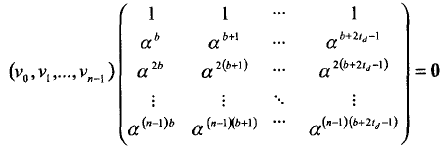
\includegraphics[scale=0.6]{chapter_2/img_08.png}
\end{center}
\end{figure}

Соответственно, проверочная матрица двоичного БЧХ кода имеет вид
\begin{figure}[htbp]
\begin{center}
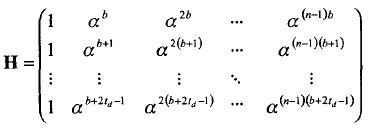
\includegraphics[scale=0.6]{chapter_2/img_09.png}
\end{center}
\end{figure}

Эта проверочная матрица обладает свойством: любая ее $2_{t_d} * 2_{t_d}$ подматрица является
\textit{матрицей Вандермонда}. Следовательно, любые $2_{t_d}$ столбцов матрицы линейно
независимы. Отсюда следует, что минимальное кодовое расстояние этого кода удовлетворяет
неравенству $d\ge 2_{t_d}+1$.

%%%%%%%%%%%%%%%%%%%%%%%%%%%%%%%%%%%%%%%%%%%%%%%%%%%%%%%%%%%%%%%%%%%%%%%%%%%%%%%%%%%%%%%%%%%
%%%%%%%%%%%%%%%%%%%%%%%%%%%%%%%%%%%%%%%%%%%%%%%%%%%%%%%%%%%%%%%%%%%%%%%%%%%%%%%%%%%%%%%%%%%
%%%%%%%%%%%%%%%%%%%%%%%%%%%%%%%%%%%%%%%%%%%%%%%%%%%%%%%%%%%%%%%%%%%%%%%%%%%%%%%%%%%%%%%%%%%
\subsection{Алгоритм кодирования БЧХ-кодом}
Кодирование БЧХ-кодом состоит из следующих операций:
\begin{enumerate}
  \item Получить вектор бит для кодирования.
  \item Преобразовать данный вектор в полином $m(x)$.
  \item Умножить полученный полином $m(x)$ на порождающий полином $g(x)$. В результате имеем полином $r(x)$.
  \item Преобразовать полученный полином $r(x)$ в вектор бит.
  \item Данный вектор бит явялется кодовым словом БЧХ-кода и передается в канал.
\end{enumerate}

%%%%%%%%%%%%%%%%%%%%%%%%%%%%%%%%%%%%%%%%%%%%%%%%%%%%%%%%%%%%%%%%%%%%%%%%%%%%%%%%%%%%%%%%%%%
%%%%%%%%%%%%%%%%%%%%%%%%%%%%%%%%%%%%%%%%%%%%%%%%%%%%%%%%%%%%%%%%%%%%%%%%%%%%%%%%%%%%%%%%%%%
%%%%%%%%%%%%%%%%%%%%%%%%%%%%%%%%%%%%%%%%%%%%%%%%%%%%%%%%%%%%%%%%%%%%%%%%%%%%%%%%%%%%%%%%%%%
\subsection{Общий алгоритм декодирования}
На Рис.~\ref{img_13} показана обобщенная структура декодера циклического кода. Синдром
$s(x)$ используется для определения полинома ошибок $e(x)$. Проблема декодирования равноценна
поиску полинома ошибок $e(x)$ по известному синдрому $s(x)$ .

\begin{figure}[htbp]
\begin{center}
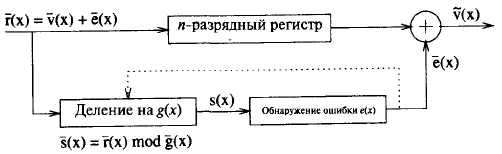
\includegraphics[scale=0.7]{chapter_2/img_13.png}
\end{center}
\caption{Обобщенная структура декодера циклического кода}
\label{img_13}
\end{figure}

%%%%%%%%%%%%%%%%%%%%%%%%%%%%%%%%%%%%%%%%%%%%%%%%%%%%%%%%%%%%%%%%%%%%%%%%%%%%%%%%%%%%%%%%%%%
%%%%%%%%%%%%%%%%%%%%%%%%%%%%%%%%%%%%%%%%%%%%%%%%%%%%%%%%%%%%%%%%%%%%%%%%%%%%%%%%%%%%%%%%%%%
%%%%%%%%%%%%%%%%%%%%%%%%%%%%%%%%%%%%%%%%%%%%%%%%%%%%%%%%%%%%%%%%%%%%%%%%%%%%%%%%%%%%%%%%%%%
\subsection{Алгоритм декодирования Берлекэмпа–Месси}
Декодирование БЧХ-кодов распадается на несколько задач. Это (1) вычисление синдромных компонент, (2) 
отыскание полинома локаторов ошибок, (3) отыскание самих локаторов ошибок как величин, обратных корням 
полинома локаторов ошибок, (4) определение величин ошибок. Архитектура БЧХ-декодера показана
на Рис.~\ref{img_11}.

\begin{figure}[htbp]
\begin{center}
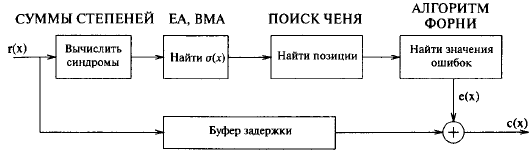
\includegraphics[scale=0.7]{chapter_2/img_11.png}
\end{center}
\caption{Архитектура БЧХ-декодера}
\label{img_11}
\end{figure}

Первоначальная версия алгоритма Берлекэмпа–Месси была изложена Берлекэмпом в 1968 году в качестве 
элемента конструкции декодера кодов Боуза–Чоудхудри–Хоквингема над конечным полем. Хотя в этой работе была 
указана возможность формулировки решаемой задачи с использованием понятия линейного регистра сдвига с 
обратной связью, алгоритм описывался исключительно в терминах полиномов и был весьма сложен для понимания. 
Спустя год Месси предложил свою интерпретацию алгоритма, как позволяющего строить линейный регистр сдвига 
минимальной длины, генерирующий заданную последовательность. Эта интерпретация оказалась полезной для более 
широкого распространения алгоритма, получившего название по имени этих двух ученых. В некоторых работах 
алгоритм излагается также с помощью непрерывных дробей и рациональной аппроксимации.

Данный алгоритм по числу операций в поле обладает высокой эффективностью и обычно рассматривается как 
итеративный процесс построения минимального линейного регистра сдвига с обратной связью. Особенностью данного 
регистра является то, что он генерирует заранее известную \emph{последовательность синдромов} $S_1, S_2, 
..., {S_2}_d$.

Алгоритм Берлекэмпа–Месси нацелен на построение многочлена $\sigma^{(l+1)}(x)$ наименьшей степени, который
удовлетворяет уравлению: $$\sum \limits_{j=0}^{l_i+1}S_{k-j}{\sigma_j}^{(i+1)}=0, l_i<k<i+1$$

Решение денной задачи эквивалентно условию, что многочен
$$\sigma^{(i+1)}(x)=1+{\sigma_1}^{(i+1)}x+\ldots+{\sigma_{l_i+1}}^{(i+1)}x^{l_{i+1}}$$

является многочленом обратной связи ЛРОС, который генерирует ограниченную последовательность синдромов.
Различие на $i$-й итерации определяется как
$$d_i=S_{i+1}+S_i\sigma_1^{(i)}+\ldots+S_{i-l_i+1}\sigma_{l_i}^{(i)}$$

является мерой соответствия синдромной последовательности и генерируемой ЛРОС и содержит корректирущий
множитель для вычисления $\sigma^{(i+1)}$ на следующей итерации. Существуют два случая:
\begin{enumerate}
\item Если $d_i=0$, то уравнение удовлетворяется неравенством.
$$\sigma{(i+1)}(x)=\sigma^1(x), l_{i+1}=l_i$$

\item Если $d\ne0$, то решение на следующей итерации имеет вид
$$\sigma^{(i+1)}(x)=\sigma^1(x)+d_i {d_m}^{-1}x^{t-m}\sigma^{(m)}(x)$$
$$l_{i+1}=max\{l_i, l_m+i-m\},$$

где является решением на $m$-й итерации такое, что $-1\le m<i$, $d_m\ne 0$, и разность $(m-l_m)$ максимальна.
Итеративное вычисление $\sigma^{(i+1)}(x)$ продолжается, пока не удовлетворится одно или оба условия: либо
$i\ge l_{i+1}+t_d-1$, либо $i=2t_d-1$.
\end{enumerate}
 
Начальные условия алгоритма:
$$\sigma^{(-1)}(x)=1, l_{-1}=0, d_{-1}=1$$
$$\sigma^{(0)}(x)=1, l_0=0, d_{0}=S_1.$$

Алгоритм Берлекэмпа–Месси можно рассматривать как итеративный процесс построения минимального линейного
регистра сдвига с обратной связью (ЛРОС), аналогично показанному на Рис.~\ref{img_12}, который
генерирует известную \textit{последовательность синдромов} $S_1, S_2, \ldots, S_{2t_d}$.

\begin{figure}[htbp]
\begin{center}
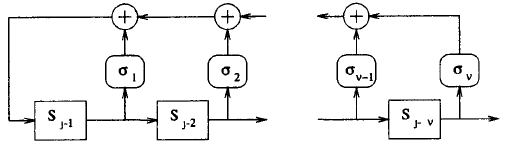
\includegraphics[scale=0.6]{chapter_2/img_12.png}
\end{center}
\caption{ЛРОС с отводами $\sigma_1, \sigma_2, \ldots, \sigma_v$}
\label{img_12}
\end{figure}

%%%%%%%%%%%%%%%%%%%%%%%%%%%%%%%%%%%%%%%%%%%%%%%%%%%%%%%%%%%%%%%%%%%%%%%%%%%%%%%%%%%%%%%%%%%
%%%%%%%%%%%%%%%%%%%%%%%%%%%%%%%%%%%%%%%%%%%%%%%%%%%%%%%%%%%%%%%%%%%%%%%%%%%%%%%%%%%%%%%%%%%
%%%%%%%%%%%%%%%%%%%%%%%%%%%%%%%%%%%%%%%%%%%%%%%%%%%%%%%%%%%%%%%%%%%%%%%%%%%%%%%%%%%%%%%%%%%
\subsection{Решение ключевого уравнения}
%\begin{definition} 
%\deft{Ключевое уравнение для задачи исправления ошибок} --- уравнение вида 
%$$\Omega(x)=S(x)\lambda(x)mod x^{d-1}$$
%где $S(x)$ --- синдромный полином, а полиномы $\lambda(x)$ и $\Omega(x)$ должны быть определены в 
%процессе декодирования, $d$ --- конструктивное расстояние.
%\end{definition}
%
%Всякий метод решения ключевого уравнения при котором по заданному $S(x)$ отыскиваются полиномы $\lambda(x)$ 
%и $\Omega(x)$ такие, что $deg\lambda(x)=t, \Omega(x)=t-1, t\le(d-1)/2$, дает некоторый метод исправления
%ошибок кратности $t$.
Если кодер передает слово двоичного БЧХ-кода
$$C(x)=\sum\limits_{i=0}^{n-1} C_i x^i,$$

а шум в канале задается вектором
$$E(x)=\sum\limits_{i=0}^{n-1} E_i x^i,$$

то полученное слово записывается многочленом
$$R(x)=\sum\limits_{i=0}^{n-1} R_i x^i=\sum\limits_{i=0}^{n-1} C_i x^i+\sum\limits_{i=0}^{n-1} E_i x^i.$$

Для $j=1, 2, \ldots, 2t$ кодовое слово кратно минимальному многочлену элемента $\alpha^j$ и, следовательно,
$$R(\alpha^j)=0+\sum\limits_{i=0}^{n-1} E_i \alpha^{ji}=S_j,$$

где элементы поля Галуа $X_1, X_2, \ldots, X_e$ -- локаторы ошибок $E_i=1$. Так как
$S_j=R(\alpha^j)=r^{(\alpha^j)}(\alpha^j)$, где $r^j(x)$ -- остаток от деления $R(x)$ на минимальный
многочлен $M^{(j)}(x)$ элемента $\alpha^j(1\le j \le 2t)$. После вычисления $S_1, S_2, \ldots, S_{2t}$
основная задача декодера -- определить $X_1, X_2, \ldots, X_e$ из уравнений
$$\sum\limits_{i=1}^{e} X_i^j=S_j,  j=1, 2, \ldots, 2t.$$

В обшщем случае эта система имеет много решений, каждое из которых соответствует различным векторам
ошибок, лежащим в одном классе смежности по аддитивной группе кодовых слов. Декодер должен найти решение
с наимешьшим возможным числом $e$.

Для решения системы декодер сначала пытается определить коэффициенты многочлена локаторов ошибок.

\begin{definition} 
$$\sigma(z)=\prod\limits_{i=1}^{e}(1-X_i z)=1+\sum\limits_{j=1}^{e}\sigma_j z^j.$$
\end{definition}

Если многочлен $\sigma(z)$ уже найден декодером, то, используя процедуру Ченя, можно найти взаимные
корни для $\sigma(z)$. Наиболее тяжелая часть этой процедуры -- определение коэффициентов $\sigma_j$
по величинам $S_j$.

Для того чтобы найти зависимость между величинами $\sigma_j$ и $S_j$, введем производящую функцию
$$S(z)=\sum\limits_{i=1}^{\infty}S_j z^j=\sum\limits_{j=1}^{\infty}\sum\limits_{i=1}^{e}X_i^j z^j=
\sum\limits_{i=1}^{e}\frac{X_{i^z}}{1-X_{i^z}}.$$

После умножения на $\sigma(z)$ имеем
$$S(z)\sigma(z)=\sum\limits_{i=1}^{e}\frac{X_{i^z}}{1-X_{i^z}}\prod\limits_{j=1}^{e}(1-X_{i^z})=
\sum\limits_{i=1}^{e}X_(i^z)\prod\limits_{j\ne i}^{}(1-X_{i^z}).$$

Прибавив к обеим частям равенства $\sigma(z)$ получим
$$[1+S(z)]\sigma(z)=\sigma(z)+\sum\limits_{i=1}^{e}X_{i^z}\prod\limits_{j\ne i}^{}(1-X_{t^z}).$$

Определим многочлен $\omega(z)=\sum\limits_{k=0}^{e}\omega_k z^k$  спомощью равенства
$$\omega(z)=\sigma(z)+\sum\limits_{k=0}^{e}X_{i^z}\prod\limits_{j\ne i}^{}(1-X_{t^z}).$$

Тогда
$$[1+S(z)]\sigma(z)=\omega(z).$$

В общем случае декодеру известны коэффициенты только при первых $2t$ степенях $z$ в $S(z)$
и не известны коэффициенты $S_{2t+1}, S_{2t+2}, S_{2t+3}, \ldots .$ Иными словами, декодер
не знает $S(z)$, но знает $S(z)mod z^{2t+1}.$ Поэтому естественно ввести уравнение, которое
мы назовем \textit{ключевым}:

$$[1+S(z)]\sigma(z)=\omega(z)mod z^{2t+1}.$$

Из этого уравнения по заданному $S(z)$ нужно найти \textit{оба} многочлена $\sigma(z)$
и $\omega(z)$, степени которых не превосходят $e$, где $e$ -- число ошибок в канале.

Одна <<физическая интерпретация>> ключевого уравнения была предложена Месси. Перепишем
уравнение в виде
$$S_k+\sum\limits_{i=1}^{k-1}\sigma_i S_{k-i}+\sigma_k=\omega_k,$$

или в виде
$$S_k=\omega_k-\sum\limits_{i=1}^{k-1}\sigma_iS_{k-i}-\sigma_k.$$

Последнее равенство задает $k$-й выход регистров сдвига, приведенных на Рис.~\ref{img_06} и Рис.~\ref{img_07}.
Обратные связи которых соответствуют многочлену $\sigma(z)$, а начальное состояние ячеек --
многочлену $\omega(z)$. 
\begin{figure}[htbp]
\begin{center}
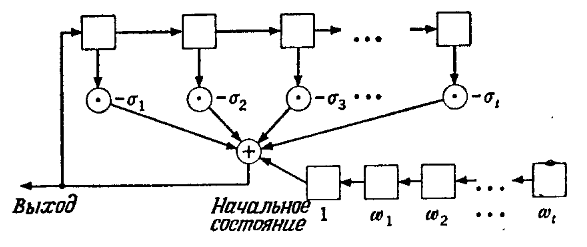
\includegraphics[scale=0.6]{chapter_2/img_06.png}
\end{center}
\caption{Интерпретация ключевого уравнения с помощью РОС}
\label{img_06}
\end{figure}

Это позволяет интерпретировать ключевое уравнение как математическую постановку задачи синтеза регистра
с обратной связью: по заданной выходной последовательности $1+S(z)$ необходимо определить обратные
связи $\sigma(z)$ и начальное состояние $\omega(z)$ кратчайшего регистра сдвига с выходной последовательностью
$1+S(z)$.

В задаче декодирования двоичных БЧХ-кодов реальный интерес представляет многочлен $\sigma(z)$, а не
многочлен $\omega(z)$. Однако это же ключевое уравнение возникает и в некоторых других приложениях.

\begin{figure}[htbp]
\begin{center}
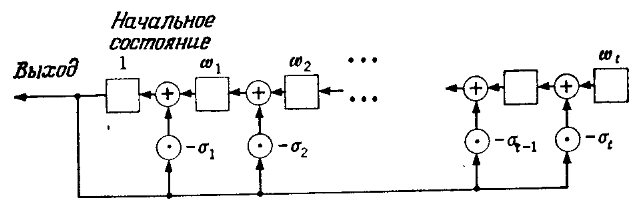
\includegraphics[scale=0.6]{chapter_2/img_07.png}
\end{center}
\caption{Другая интерпретация ключевого уравнения с помощью РОС}
\label{img_07}
\end{figure}

%%%%%%%%%%%%%%%%%%%%%%%%%%%%%%%%%%%%%%%%%%%%%%%%%%%%%%%%%%%%%%%%%%%%%%%%%%%%%%%%%%%%%%%%%%%
%%%%%%%%%%%%%%%%%%%%%%%%%%%%%%%%%%%%%%%%%%%%%%%%%%%%%%%%%%%%%%%%%%%%%%%%%%%%%%%%%%%%%%%%%%%
%%%%%%%%%%%%%%%%%%%%%%%%%%%%%%%%%%%%%%%%%%%%%%%%%%%%%%%%%%%%%%%%%%%%%%%%%%%%%%%%%%%%%%%%%%%
\subsection{Вычисление синдромов}
Синдромы вычисляются как значения принятого полнинома в нулях кода
\footnote{Для двоичных БЧХ кодов справедливо равенство $S_{2i}=S_i^2$, которое
позволяет сократить объем вычислений.}
$$S_i=r(\alpha^i), i=b, b+1, \ldots, b+2t_d -1$$

Вычисление синдромов может быть реализовано аппаратно. На Рис.~\ref{img_10} показан
пример схемы аппаратного вычисления синдрома.
\begin{figure}[htbp]
\begin{center}
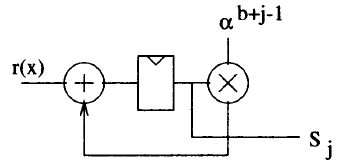
\includegraphics[scale=0.6]{chapter_2/img_10.png}
\end{center}
\caption{Пример вычисления синдрома}
\label{img_10}
\end{figure}

%%%%%%%%%%%%%%%%%%%%%%%%%%%%%%%%%%%%%%%%%%%%%%%%%%%%%%%%%%%%%%%%%%%%%%%%%%%%%%%%%%%%%%%%%%%
%%%%%%%%%%%%%%%%%%%%%%%%%%%%%%%%%%%%%%%%%%%%%%%%%%%%%%%%%%%%%%%%%%%%%%%%%%%%%%%%%%%%%%%%%%%
%%%%%%%%%%%%%%%%%%%%%%%%%%%%%%%%%%%%%%%%%%%%%%%%%%%%%%%%%%%%%%%%%%%%%%%%%%%%%%%%%%%%%%%%%%%
\subsection{Граница Синглтона}
\textbf{Определение}

Граница Синглтона (названная в честь Р. К. Синглтона) устанавливает предел мощности кода $C$ 
с символами из поля $\mathbb{F}_q$ длины $n$ и минимального расстояния Хэмминга $d$.  

Пусть $A_q(n,d)$ обозначает максимально возможную мощность $q$-ичного кода длины $n$
($q$-ичный код — это код над полем из $q$ элементов). Пусть минимальное расстояние Хэмминга
между двумя словами кода будет $d$, то есть $\mathrm D_H(w,\;w')\geqslant d$ для любых двух
кодовых слов $w$ и $w'$. 

Тогда : $A_q(n,\;d)\leqslant q^{n-d+1}.$

\textbf{Доказательство}

В первую очередь заметим, что верхняя граница максимальной мощности любого $q$-ичного кода
длины $n$ равняется $q^n$, так как каждый компонент данного кодового слова может принимать
одно из $q$ разных значений независимо от других компонентов.

Пусть $C$ является $q$-ичным кодом. Тогда все слова $c \in C$ в кодe отличны друг от друга.
Если мы сотрём первые $d-1$ символов каждого слова, тогда все оставшиеся кодовые слова должны
оставаться разными, так как расстояние Хэмминга между словами кода $C$ по меньшей мере $d$.
Следовательно мощность кода после удаления $d-1$ символов осталась прежней.

Длина нового кода
$$n-(d-1)=n-d+1,$$

и следовательно максимально возможной мощностью такого кода является $q^{n-d+1}.$

Отсюда следует верхняя граница мощности и для изначального кода
$$A_q(n,\;d)\leqslant q^{n-d+1}.$$

\textbf{Линейные коды}

В случае с линейными кодами можно записать границу Синглтона как
$$q^k\leqslant q^{n-d+1}$$

или
$$k\leqslant n-d+1.$$

Линейные коды, для которых выполняется равенство $k=n-d+1$, называются \textit{разделимыми
кодами с максимальным расстоянием} или кодами МДР. Известными представителями этого семейства
кодов являются \textit{код Рида — Соломона} и коды, образуемые из него.

%%%%%%%%%%%%%%%%%%%%%%%%%%%%%%%%%%%%%%%%%%%%%%%%%%%%%%%%%%%%%%%%%%%%%%%%%%%%%%%%%%%%%%%%%%%
%%%%%%%%%%%%%%%%%%%%%%%%%%%%%%%%%%%%%%%%%%%%%%%%%%%%%%%%%%%%%%%%%%%%%%%%%%%%%%%%%%%%%%%%%%%
%%%%%%%%%%%%%%%%%%%%%%%%%%%%%%%%%%%%%%%%%%%%%%%%%%%%%%%%%%%%%%%%%%%%%%%%%%%%%%%%%%%%%%%%%%%
\section{Сверточные коды}

\begin{definition} 
\deft{Сверточные кодирование} --- метод кодирования, при котором каждый символ входной последовательности, 
состоящей из $k$ битов, преобразуется в $n$-битовый кодированный поток данных. Внесение избыточности и 
соответственное увеличение скорости передачи в $n/k$ раз, позволяет повысить помехоустойчивость, особенно в 
каналах с одиночными ошибками.
\end{definition}

\subsection{Алгоритм кодирования сверточным кодом}
Алгоритм основан на работе сверточного кодера. Кодер имеет набор входов и выходов. Символы информационной
последовательности поступают на вход кодера и попадают в регистр сдвига с обратной связью. В результате
выполения операции сдвига на выходах кодера появляются выходные символы, которые и формируют кодовые слова.

Сверточный кодер представлен на Рис.~\ref{img_02}.

\begin{figure}[htbp]
\begin{center}
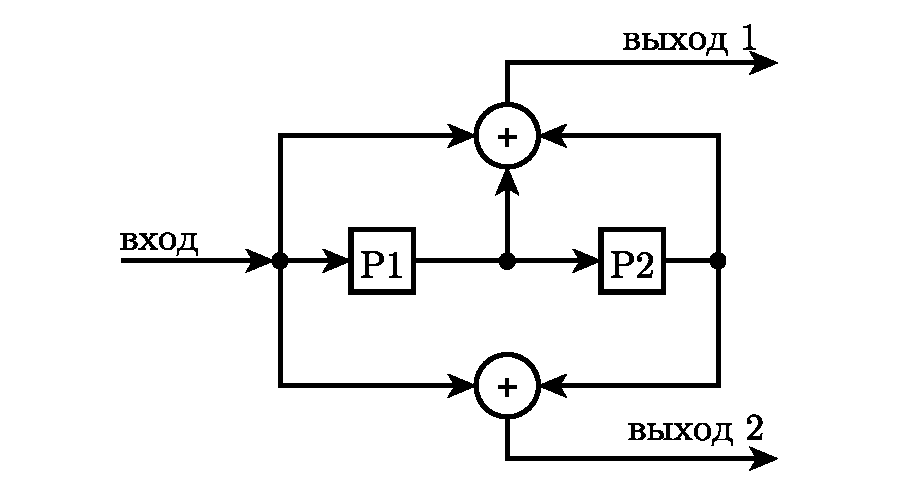
\includegraphics[scale=0.6]{chapter_2/img_02.pdf}
\end{center}
\caption{Сверточный кодер}
\label{img_02}
\end{figure}

%%%%%%%%%%%%%%%%%%%%%%%%%%%%%%%%%%%%%%%%%%%%%%%%%%%%%%%%%%%%%%%%%%%%%%%%%%%%%%%%%%%%%%%%%%%
%%%%%%%%%%%%%%%%%%%%%%%%%%%%%%%%%%%%%%%%%%%%%%%%%%%%%%%%%%%%%%%%%%%%%%%%%%%%%%%%%%%%%%%%%%%
%%%%%%%%%%%%%%%%%%%%%%%%%%%%%%%%%%%%%%%%%%%%%%%%%%%%%%%%%%%%%%%%%%%%%%%%%%%%%%%%%%%%%%%%%%%
\subsection{Алгоритм Витерби}
Классическим методом коррекции ошибок, по праву считавшимся лучшим в течение нескольких десятилетий, является 
декодер Витерби, применяемый для декодирования сверточных кодов. Данный алгоритм является оптимальным и легко 
реализуемым для коротких сверточных кодов. В связи с этим сверточные коды, декодируемые с помощью алгоритма 
Витерби, применяются в большинстве стандартов систем передачи данных, например, в беспроводных сетях 
стандартов IEEE 802.11, IEEE 802.16, дальней космической связи CCSDS, спутниковой связи TIA-1008 и др. 
Использование длинных (с конструктивной длиной более 9) и потенциально более эффективных кодов в декодере 
Витерби представляется нецелесообразным из-за экспоненциального роста сложности его реализации от длины кода. 
Поэтому долгое время усилия многих специалистов были направлены на разработку алгоритмов декодирования, 
которые способны эффективно декодировать длинные коды при небольшой сложности реализации.

В основе алгоритм Витерби лежит принцип максимума правдоподобия. В процессе декодирования кодового слова
декодер Витерби находит кодовую последовательность, ближайшую к принятой. 

\begin{enumerate}
\item Вычисление метрик рёбер решётки. Метрика ребра решётки на вычисляется как Хэмминговое расстояние
между меткой ребра и двоичной последовательностью на входе декодера. Расстояние между последовательностями
по Хэммингу --- количество различающихся битов в последовательностях.
\item Прибавить, сравнить, выбрать.
Для каждого состояния и соответствующей пары рёбер, входящих в данное состояние из двух возможных
предшествующих, вычислить и сравнить следующие суммы. Выбрать ребро с меньшей суммой.
\item Декодирование символов.
Вычислить декодируемый символ и записать его в буфер накопленной последовательности. При этом выдать
ранее сохраненный символ на выход декодера.
\end{enumerate}

Особенностью Декодер Витерби является то, что при последовательном декодировании при возникновении
ошибок в канале метрики путей растут. Для устранения этого недостатка выполняется процедура
нормализации метрик. Существует два способа нормализации метрик: пороговый и модулярный.

Пример декодирования кодового слова с использованием алгоритма Витерби приведен на на Рис.~\ref{img_03}.

\begin{figure}[htbp]
\begin{center}
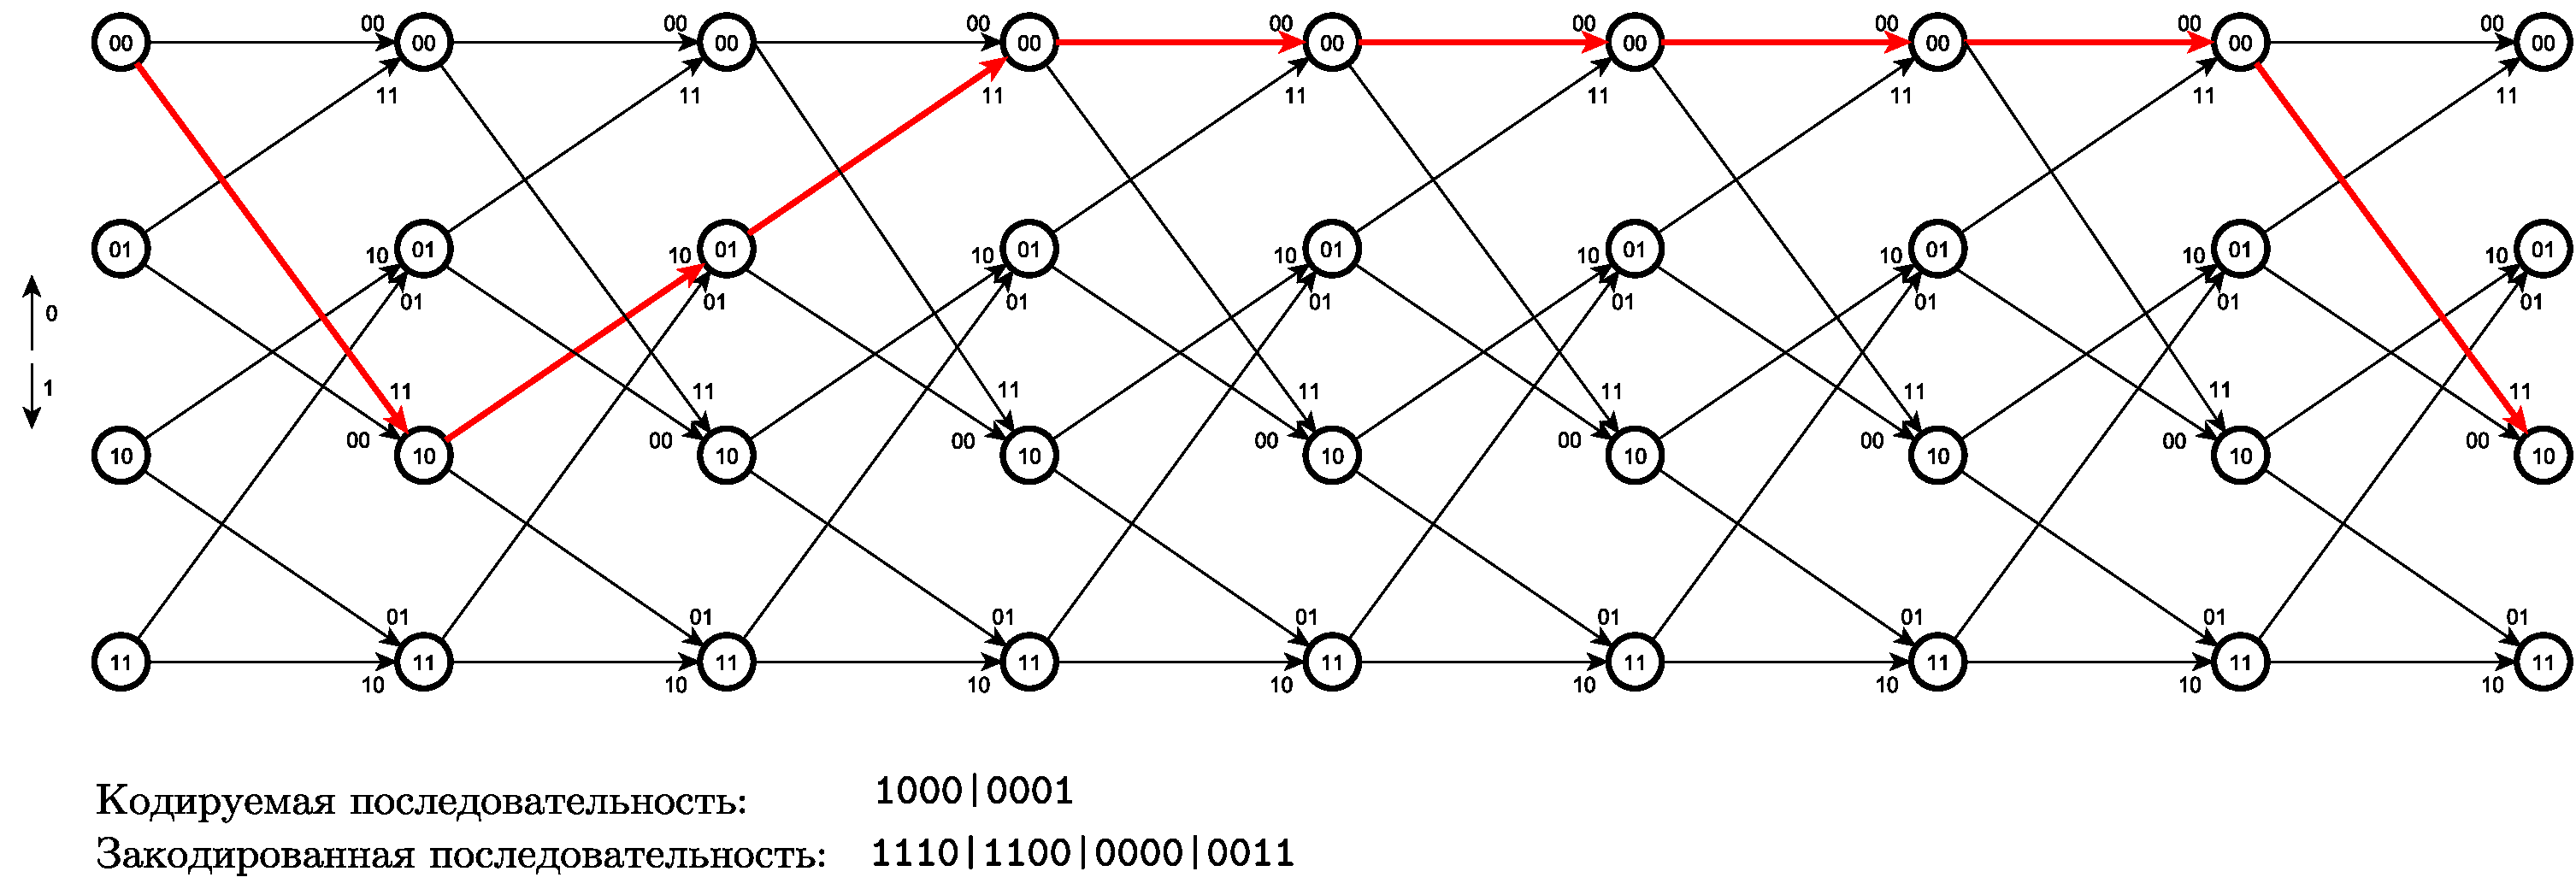
\includegraphics[scale=0.3]{chapter_2/img_03.pdf}
\end{center}
\caption{Декодирование кодового слова с использованием алгоритма Витерби}
\label{img_03}
\end{figure}

%%%%%%%%%%%%%%%%%%%%%%%%%%%%%%%%%%%%%%%%%%%%%%%%%%%%%%%%%%%%%%%%%%%%%%%%%%%%%%%%%%%%%%%%%%%
%%%%%%%%%%%%%%%%%%%%%%%%%%%%%%%%%%%%%%%%%%%%%%%%%%%%%%%%%%%%%%%%%%%%%%%%%%%%%%%%%%%%%%%%%%%
%%%%%%%%%%%%%%%%%%%%%%%%%%%%%%%%%%%%%%%%%%%%%%%%%%%%%%%%%%%%%%%%%%%%%%%%%%%%%%%%%%%%%%%%%%%
\section{Каскадные коды}
Каскадные коды используются в практике передачи дискретных сигналов в качестве методов реализации кодов 
большой длины и высокой корректирующей способности. Эта цель может быть достигнута применением нескольких 
ступеней кодирования; наибольшее распространение получили две ступени кодирования различными кодами, например 
по схеме, показанной на Рис.~\ref{img_04}.

\begin{figure}[htbp]
\begin{center}
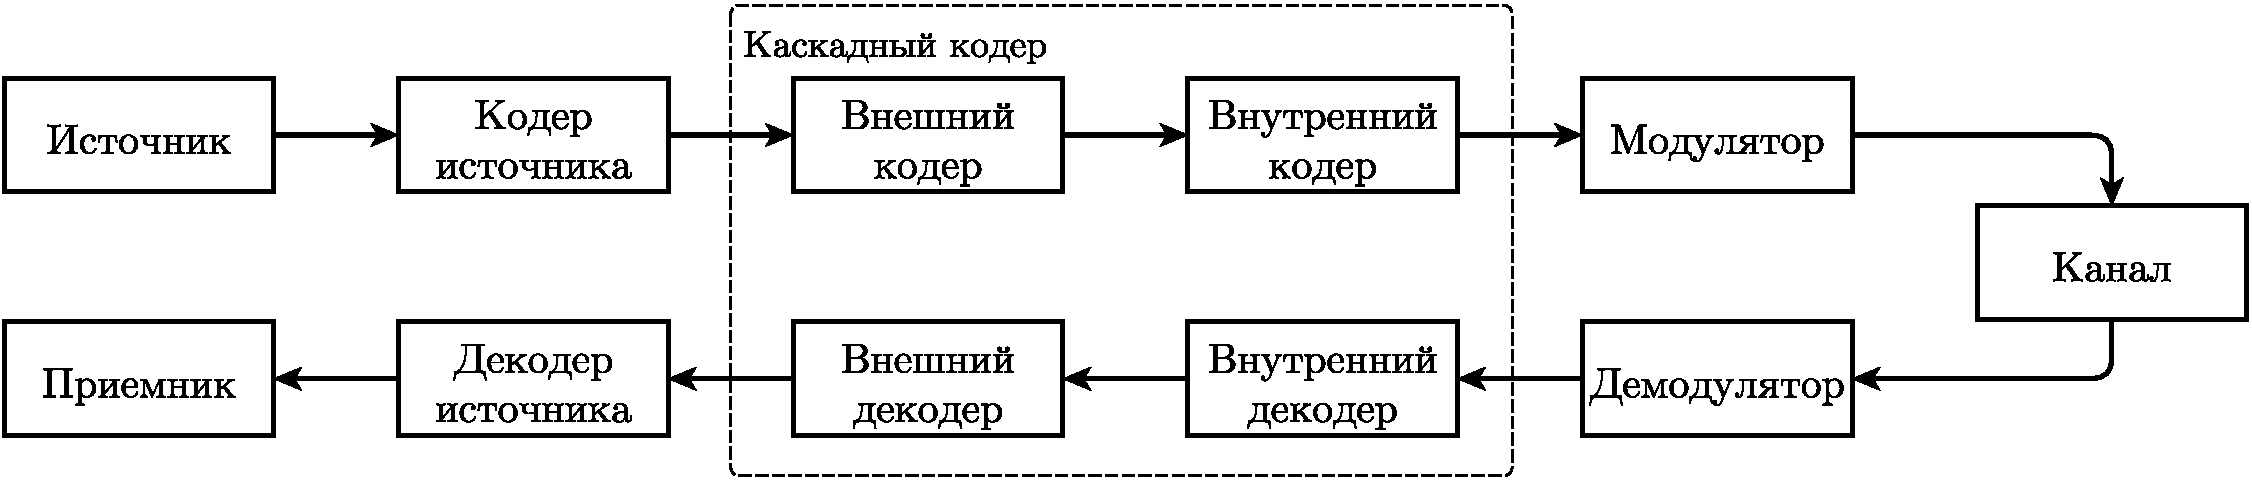
\includegraphics[scale=0.4]{chapter_2/img_04.pdf}
\end{center}
\caption{Cистема передачи информации при использовании каскадного кодирования}
\label{img_04}
\end{figure}

Поступающие от источника сообщений данные разбиваются на блоки из $К$ недвоичных ($m$-ичных) символов, 
содержащие $k$ информационных элементов ($k=km$), которые кодируются недвоичным $(n, k)$кодом. Очевидно, что 
каждый коэффициент $(n, k )$ кода cодержит $m$ двоичных элементов. Последовательность $(n, k)$ кода, 
состоящая из $n_1=nm$ двоичных элементов поступает на внутренний кодер, где разбивается на $m$-элементные 
блоки, которые кодируются внутренним $(n_2, m)$ кодом. Число кодовых комбинаций $N=K+R$, поэтому на выходе 
внутреннего кодера число двоичных элементов будет $n=n_2*N$.

%%%%%%%%%%%%%%%%%%%%%%%%%%%%%%%%%%%%%%%%%%%%%%%%%%%%%%%%%%%%%%%%%%%%%%%%%%%%%%%%%%%%%%%%%%%
%%%%%%%%%%%%%%%%%%%%%%%%%%%%%%%%%%%%%%%%%%%%%%%%%%%%%%%%%%%%%%%%%%%%%%%%%%%%%%%%%%%%%%%%%%%
%%%%%%%%%%%%%%%%%%%%%%%%%%%%%%%%%%%%%%%%%%%%%%%%%%%%%%%%%%%%%%%%%%%%%%%%%%%%%%%%%%%%%%%%%%%
\subsection{Получение каскадных кодов}
Схема системы передачи информации, используемая для анализа кодов в данной работе представлена на
Рис.~\ref{img_05}.

\begin{figure}[htbp]
\begin{center}
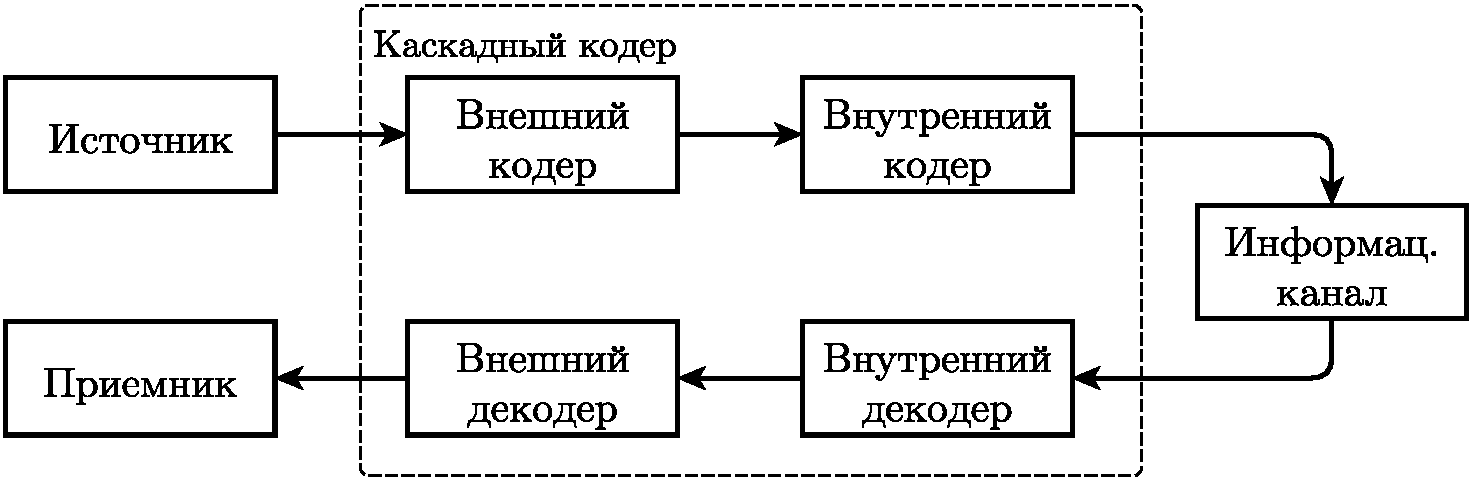
\includegraphics[scale=0.4]{chapter_2/img_05.pdf}
\end{center}
\caption{Cистема передачи информации для анализа кодов}
\label{img_05}
\end{figure}

В данной работе внешним кодером выступает БЧХ-кодер, который генерирует кодовое слово БЧХ-кода c параметрами 
$(15, 5, 7 )$. Установлено, что данный код гарантированно исправляет ошибки в количестве $t\le3$. Указанное 
слово поступает на вход внутреннего кодера, которым является сверточный кодер. Он принимает кодовое слово БЧХ
-кода и кодирует его в слово сверточного кода с параметрами $(2, 1)$. На выходе получаем кодовые слова 
сверточного кода, которые поступают в модулятор. В данной работе модулятор не используется по причине 
акцента внимания на анализ кодов. Таким образом, кодовые слова сверточного кода поступают в информационный 
канал, где происходит их искажение.

%%%%%%%%%%%%%%%%%%%%%%%%%%%%%%%%%%%%%%%%%%%%%%%%%%%%%%%%%%%%%%%%%%%%%%%%%%%%%%%%%%%%%%%%%%%
%%%%%%%%%%%%%%%%%%%%%%%%%%%%%%%%%%%%%%%%%%%%%%%%%%%%%%%%%%%%%%%%%%%%%%%%%%%%%%%%%%%%%%%%%%%
%%%%%%%%%%%%%%%%%%%%%%%%%%%%%%%%%%%%%%%%%%%%%%%%%%%%%%%%%%%%%%%%%%%%%%%%%%%%%%%%%%%%%%%%%%%
\subsection{Декодирование каскадных кодов}
При декодировании каскадного кода выполняется ряд обратных кодированию процедур. Так, при демодуляции на 
удаленной стороне имеем кодовое слово сверточного кода. Данное слово декодируется сверточным декодером, 
который построен на основе алгоритма Витерби. В результате декодирования нескольких кодовых слов имеем 
кодовое слово БЧХ-кода, которое подается на вход БЧХ-декодеру. В результате декодирования данного слова 
имеем исходные данные, то есть данные сгенерированные кодером источника.  Очевидно, что принцип каскадного 
декодирования аналогичен действию получателя искаженной телеграммы. Так, если искажены буквы в словах (
независимые ошибки в канале), то они могут быть обнаружены и исправлены с помощью других букв того же слова (
внутреннее кодирование решает эту задачу), а если же отдельные слова искажены до неузнаваемости ( 
группирующиеся ошибки пакеты), то обнаруженное наличие таких ошибок и тем более их исправление возможно 
только с помощью других слов предложения или текста в целом (внешнее кодирование). В рассмотренной аналогии 
основу внутреннего кода составляет избыточность за счет связей между буквами в словах, а внешнего кода за 
счет связей слов в предложении.
\chapter{Описание программной модели}
\section{Общие сведения}
Программная модель представляет собой консольное приложение, предназначенное для моделирования и анализа 
системы передачи данных при использовании каскадных кодов. Приложение имеет интерфейс командной строки и 
позволяет выполнять конфигурацию модели перед ее запуском путем указания параметров используемых кодов. В 
случае, если данные параметры не указываются, модель конфигурируется параметрами по умолчанию. Полный набор 
опций разработанной модели представлен в Листинге~\ref{lst_01}.

\begin{lstlisting}[caption={Вывод информации о доступных опциях}, label={lst_01}]
Administrator@DNAPC /cygdrive/d/SUAI/8sem/Alexeev/msvs10/scm_new/csm/build/bin/Release/app
$ ./app --h
Usage: csm [-uv] [-g <int>] [-l <int>] [-e <int>] [-d <int>] [-b <double>] [-p <string>] <file> [<file>]... [--help] [--version]
Program performs simulation of data transfer in communication system. The system is structured in the following manner:
[Transmitter]->[BCH encoder]->[Convolutional Encoder]->[Binary Symmetric Channel]->[Viterbi Decoder]->[BCH decoder]->[Receiver]
The following options are available:
  -g, --galois=<int>        define Evariste Galois field degree (between 2..20, default is 4)
  -l, --length=<int>        define BCH code length (default is 15)
  -e, --errors=<int>        define BCH code error correction property (default is 3)
  -d, --dbuffer=<int>       define internal buffer size of trellis node in Viterbi Decoder (default is 2 frames)
  -b, --ber=<double>        define channel Bit Error Rate (default is 1e-12)
  -p, --postfix=<string>    define out file postfix (default is 'transferred')
  <file>                    define input file(s)
  -u, --gui                 run under GUI
  -v, --verbose, --debug    verbose messages
  --help                    print this help and exit
  --version                 print version information and exit
\end{lstlisting}

В качестве исходного файла, предназначенного для его использования при моделировании процесса передачи 
данных, указывается потенциально любой файл. Следует учесть, что в случае, если исходный файл имеет размер, 
больший чем 1МБ, то процесс моделирования затянется на достаточное время. Это связано с тем, что при 
реализации данной модели акцент на оптимизацию по времени выполнения прочеса симуляции, размеру потребляемой 
памяти приложением, оценке производительности приложения в целом, не делался. Главной задачей было убедиться 
в работоспособности модели для получения с нее результатов моделирования.

\section{Используемый инcтрументарий и техника разработки}
При построении модели системы передачи информации использовалась интегрированная среда разработки Microsoft 
Visual Studio 2010. Разработка велась преимущественно на языке высокого уровня С с добавлением конструкций, 
характерных для языка С++. При построении модели применялось компонентно-ориентированное программирование --- 
парадигма программирования, ключевой фигурой которой является компонент. В качестве такого компонента 
выступает библиотека, реализующая необходимый функционал, и обладающая своим интерфейсом. Несмотря на широкое 
использование данного подхода при построении систем на С++, указанный подход являлся основой для построения 
системы в целом. В результате изменения в существующую систему вносятся путём создания новых компонентов в 
дополнение или в качестве замены ранее существующих. Особое значение было уделено интерфейсам компонентов и 
технике, позволяющей строить гибкие системы и использовать большинство широко распространенных паттернов 
проектирования в случае использования языка С.

При реализации модели автор старался применять разработку через тестирование (test-driven development, TDD) и 
модульное тестирование --- техники разработки программного обеспечения, которые основываются на повторении 
очень коротких циклов разработки. Ключевыми моментами являются частые релизы, рефакторинг, контроль 
архитектуры.

\section{Архитектура модели}
Модель реализуется в виде набора компонентов, представленных в виде статических библиотек, каждая из которых 
решает свою, четко обозначенную задачу. Так, в проекте используются библиотеки, предназначенные для 
кодирования/декодирования БЧХ-кодов, кодирования/декодирования сверточных кодов. Характерной особенностью 
является разнесение ответственности компонентов и разбиение кодеров и декодеров на кодеры переднего плана и 
кодеры заднего плана. Такая практика позволяет контролировать архитектуру отдельных компонентов библиотеки и 
гибко управлять интерфейсом компонентов. Более того, практика дает возможность гибкого модифицирования или же 
замены алгоритма работы компонента заднего плана. Помимо этого, имеются библиотеки, служащие для 
моделирования канала передачи данных, тестового окружения.

\chapter{Запуск программной модели}
Генерируемая инормация после после окончания моделирования представлена в Листинге~\ref{lst_02}.
Характерной особенностью является автоматическое тестирвоание на предмет корректности принятых данных
на удаленной стороне.

\begin{lstlisting}[caption={Вывод информации после окончания моделирования}, label={lst_02}]
Administrator@DNAPC /cygdrive/d/SUAI/8sem/Alexeev/msvs10/scm_new/TeX/inc/img/chapter_4
$ ./app -b 0.0001 img_test_01.gif
Performing 'img_test_01.gif'
Progress: 100%

... transmitter stopped
... transmitter settings ...
data size: 156456
frame size: 5
... transmitter statistics ...
transmitted frames: 31292
transmitted bits: 156460

... receiver stopped
... receiver settings ...
data size: 156456
frame size: 5
... receiver statistics ...
received frames: 31292
valid frames: 31292 (100.00%)
invalid frames: 0 (0.00%)
received bits: 156460
valid bits: 156460 (100.00%)
invalid bits: 0 (0.00%)
BER: 0.000000
FER: 0.000000

... bch encoder stopped
... bch encoder settings ...
galois field degree: 4
code length: 15
information symbols quantity: 5
error correction property: 3
... bch encoder statistics ...
encoded frames: 31292
generated codewords: 31292
transmitted bits: 469380

... bch decoder stopped
... bch decoder settings ...
galois field degree: 4
code length: 15
information symbols quantity: 5
error correction property: 3
... bch decoder statistics ...
received bits: 469380
received bits (valid): 469380
received bits (corrupted): 0
received codewords: 31292
received codewords (valid): 31292
received codewords (corrupted): 0
generated frames: 31292

... cnv encoder stopped
... cnv encoder settings ...
quantity of registers: 2
codeword length: 30
... cnv encoder statistics ...
encoded frames: 31292
generated codewords: 31292
transmitted bits: 938760

... cnv decoder stopped
... cnv decoder settings ...
decoded sequence buffer size: 31
... cnv decoder statistics ...
delayed frames: 2
received bits: 938820
received bits (valid): 935880
received bits (corrupted): 98
received codewords: 31294
received codewords (valid): 31196
received codewords (corrupted): 98
generated frames: 31294

... channel bs stopped
... channel bs settings ...
BER: 0.000100
... channel bs statistics ...
bits transferred: 938820
bits corrupted: 98 (0.01%)
test: OK
\end{lstlisting}

%%%%%%%%%%%%%%%%%%%%%%%%%%%%%%%%%%%%%%%%%%%%%%%%%%%%%%%%%%%%%%%%%%%%%%%%%%%%%%%%%%%%%%%%%%%
%%%%%%%%%%%%%%%%%%%%%%%%%%%%%%%%%%%%%%%%%%%%%%%%%%%%%%%%%%%%%%%%%%%%%%%%%%%%%%%%%%%%%%%%%%%
%%%%%%%%%%%%%%%%%%%%%%%%%%%%%%%%%%%%%%%%%%%%%%%%%%%%%%%%%%%%%%%%%%%%%%%%%%%%%%%%%%%%%%%%%%%
\chapter{Результаты моделирования}
Данный раздел содержит результаты моделирвоания передачи данных при использовании каскадного
кодирования. Моделирование выполнялось с использованием разработанного и протестированного
приложения. Основная цель моделирования --- получение наглядных результатов, демонстрирующих
эффективность каскадного кодирования и корреллирующих с теоретическими ожиданиями, а также
оценка частоты появления ошибок на удаленной стороне.

%%%%%%%%%%%%%%%%%%%%%%%%%%%%%%%%%%%%%%%%%%%%%%%%%%%%%%%%%%%%%%%%%%%%%%%%%%%%%%%%%%%%%%%%%%%
%%%%%%%%%%%%%%%%%%%%%%%%%%%%%%%%%%%%%%%%%%%%%%%%%%%%%%%%%%%%%%%%%%%%%%%%%%%%%%%%%%%%%%%%%%%
%%%%%%%%%%%%%%%%%%%%%%%%%%%%%%%%%%%%%%%%%%%%%%%%%%%%%%%%%%%%%%%%%%%%%%%%%%%%%%%%%%%%%%%%%%%
\section{Передача изображения по системе моделирования}
На Рис.~\ref{img:experimoriginal} -- \ref{img:experimcoded12} представлены исходное изображение, моделирование передачи которого
производилось на программной модели. На вход поступают данные изображения, затем они искажаются в канале
в зависимости от текущих параметров канала. Далее искаженные данные принимаются на удаленной стороне и
декодируются. Под каждым изображением указаны параметры модели. Нотация параметров коррелирует с обозначением
ключей приложения, реализующего программную модель.

\begin{figure}[h]
\begin{center}
\begin{minipage}[h]{0.4\linewidth}
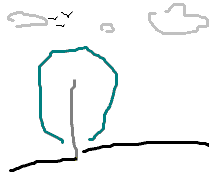
\includegraphics[width=1\linewidth]{chapter_4/img_test_06.png}
\caption{Исходное изображение} %% подпись к рисунку
\label{img:experimoriginal} %% метка рисунка для ссылки на него
\end{minipage}
\hfill 
\begin{minipage}[h]{0.4\linewidth}
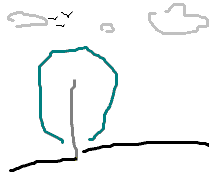
\includegraphics[width=1\linewidth]{chapter_4/img_test_06_transferred_g_4_l_15_e_3_d_31_b_0_000024.png}
\caption{g=4, l=15, e=3, d=31, b=0.000024}
\label{img:experimcoded2}
\end{minipage}
\end{center}

\begin{center}
\begin{minipage}[h]{0.4\linewidth}
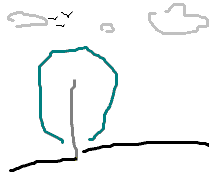
\includegraphics[width=1\linewidth]{chapter_4/img_test_06_transferred_g_4_l_15_e_3_d_31_b_0_009844.png}
\caption{g=4, l=15, e=3, d=31, b=0.009844}
\label{img:experimcoded3}
\end{minipage}
\hfill 
\begin{minipage}[h]{0.4\linewidth}
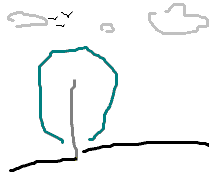
\includegraphics[width=1\linewidth]{chapter_4/img_test_06_transferred_g_4_l_15_e_3_d_31_b_0_011813.png}
\caption{g=4, l=15, e=3, d=31, b=0.011813}
\label{img:experimcoded4}
\end{minipage}
\end{center}
\end{figure}

\begin{figure}[h]
\begin{center}
\begin{minipage}[h]{0.4\linewidth}
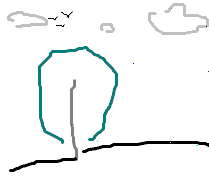
\includegraphics[width=1\linewidth]{chapter_4/img_test_06_transferred_g_4_l_15_e_3_d_31_b_0_029395.png}
\caption{g=4, l=15, e=3, d=31, b=0.029395}
\label{img:experimcoded9}
\end{minipage}
\hfill 
\begin{minipage}[h]{0.4\linewidth}
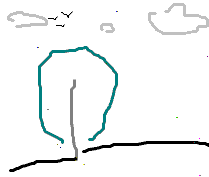
\includegraphics[width=1\linewidth]{chapter_4/img_test_06_transferred_g_4_l_15_e_3_d_31_b_0_035275.png}
\caption{g=4, l=15, e=3, d=31, b=0.035275}
\label{img:experimcoded10}
\end{minipage}
\end{center}

\begin{center}
\begin{minipage}[h]{0.4\linewidth}
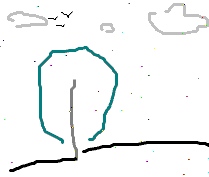
\includegraphics[width=1\linewidth]{chapter_4/img_test_06_transferred_g_4_l_15_e_3_d_31_b_0_042329.png}
\caption{g=4, l=15, e=3, d=31, b=0.042329}
\label{img:experimcoded11}
\end{minipage}
\hfill 
\begin{minipage}[h]{0.4\linewidth}
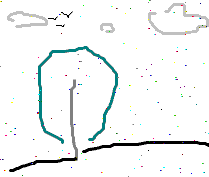
\includegraphics[width=1\linewidth]{chapter_4/img_test_06_transferred_g_4_l_15_e_3_d_31_b_0_060954.png}
\caption{g=4, l=15, e=3, d=31, b=0.060954}
\label{img:experimcoded12}
\end{minipage}
\end{center}
\end{figure}

Из данных рисунков видно, что приемлeмое качество изображения сохраняется даже при $BER=0.017011$, что говорит
о эффективности методов каскадного кодирования. При использовании $BER=0.020413$ изображение начинает содержать
искажения, которые увеличиваются при увеличении $BER$ соответственно. В реальной жизни, как правило, уровень ошибок в канале связи
гораздо меньше указанных значений (обычно он меньше $10^{-5}$). Это означает, что принятое изображение будет в таком случае примлемого
качества и пользователь на удаленной стороне практически не заметит разницу в случае, если даже при декодировании не удалось
восстановить исходную информацию.

%%%%%%%%%%%%%%%%%%%%%%%%%%%%%%%%%%%%%%%%%%%%%%%%%%%%%%%%%%%%%%%%%%%%%%%%%%%%%%%%%%%%%%%%%%%
%%%%%%%%%%%%%%%%%%%%%%%%%%%%%%%%%%%%%%%%%%%%%%%%%%%%%%%%%%%%%%%%%%%%%%%%%%%%%%%%%%%%%%%%%%%
%%%%%%%%%%%%%%%%%%%%%%%%%%%%%%%%%%%%%%%%%%%%%%%%%%%%%%%%%%%%%%%%%%%%%%%%%%%%%%%%%%%%%%%%%%%
\section{Оценка частоты появления ошибок на удаленной стороне}
На Рис.~\ref{dependencies_all} показаны графики зависимостей логарифмическом масштабе $BER$ на приемнике от $BER$ в канале при условии,
что размер буфера накопленной последовательности в узле решетки декодера Витерби составляет 1-10 фреймов (1 фрейм состоит из 15 символов).

Для получения теоретических результатов и сравнения с ними результатов, полученных на практике был выполнен следующий
эксперимент. Выполнялось моедлирование передачи данных при отключенном БЧХ-кодировании/декодировании, то есть использовалось
только сверточное кодирование и декодирование по алгоритму Витерби. Данная конфигурация обусловлена тем, что достаточно
просто (для использовавшегося сверточного кодера) построить верхнюю оценку зависимости $BER$ на приемнике от $BER$ в канале.

График черного цвета показывает кривую,
получающуюся в результате теоретических вычислений. Из данного рисунка можно наблюдать, что теоретический результат
(верхняя граница) близок к результатам, полу-ченным благодаря моделированию.
\begin{figure}[h]
\begin{center}
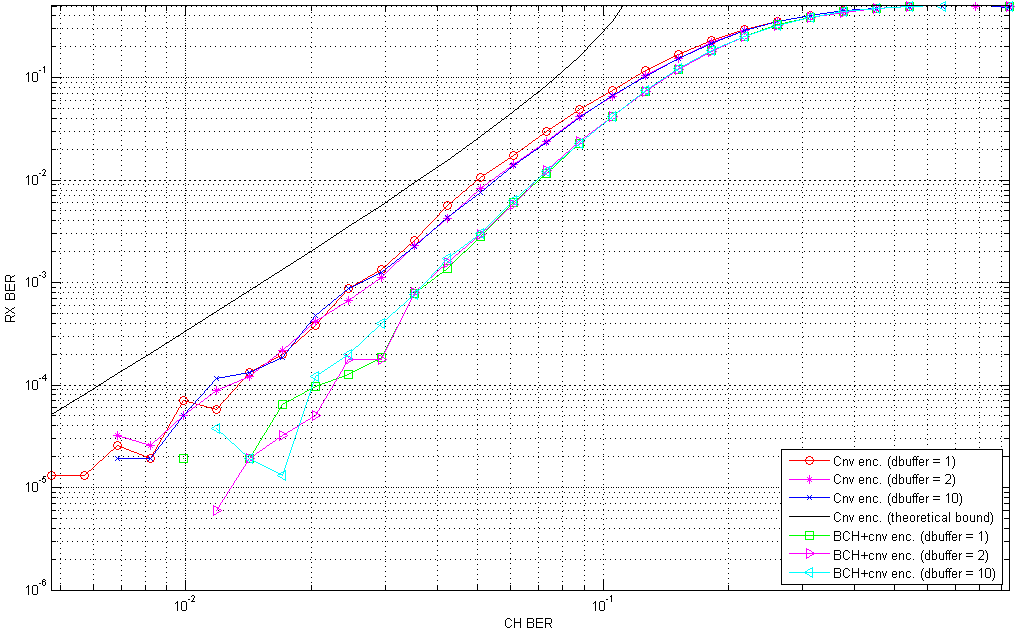
\includegraphics[width=0.9\linewidth]{chapter_4/matlab_img/dependencies_all.png}
\caption{Зависимости BER на приемнике от BER в канале}
\label{dependencies_all}
\end{center}
\end{figure}

Данный результат полностью согласуется с теорией. Более того, по предыдущим иллюстрациям можно наблюдать, что
зависимость уменьшения $BER$ на приемнике от применения буфера накопленной последовательности в узле решетки
декодера Витерби большего размера сохраняется.
% Здесь заканчивается нумерованная часть документа и начинаются ссылки и заключение
\backmatter
\Conclusion % заключение к отчёту
Представленная работа посвящена реализации и исследованию модели системы передачи информации при использовании каскадных кодов (коды 
БЧХ и сверточные коды). Указанная модель системы была реализована в виде набора независимых компонентов, каждый из которых был 
тщательно отлажен. По завершению этапа построения и реализации модели она была использована для имитационного моделирования процесса 
передачи данных изображения по системе для наглядной демонстрации результатов передачи данных и эффективности каскадного кодирования и 
для оценки зависимости $BER$ на приемнике от $BER$ в канале. Выполнялось имитационное моделирование при отключенном механизме БЧХ-
кодирования/декодирования для получения теоретических результатов и сравнения с ними результатов, полученных на практике в предыдущем 
случае.

Были получены результаты, которые показали, что сверточное кодирование и использование алгоритма Витерби при декодировании позволяют 
получать данные (изображения) приемлемого качества даже при значении $BER$ в канале, равном $BER=0.017011$. По сравнению с аналогичным 
значением в реальных физических каналах (не более $10^{-5}$) данный результат говорит о эффективности применения сверточного 
кодирования.

Использование БЧХ-кодирования позволяет восстанавливать информацию, которую не смог восстановить декодер Витерби. В реальных же 
системах, внешний декодер исправляет пакеты ошибок, которые генерирует декодер Витерби, в случае, если он не в состоянии исправить их. 
Таким образом совместное использование указанных способов кодирования позволяет повысить надежность передачи данных.

Другой результат связан с определением оптимального размера буфера накопленной последовательности узла решетки, которая применяется в 
декодере, работающем по алгоритму Витерби. Экспериментальные исследования показали, что действительно, увеличение размера указанного 
буфера позволяет получить выигрыш. Однако, чем больше буфер, тем меньше заметен выигрыш и при разработке реального устройства 
необходимо учитывать экономическую составляющую. Например, стоимость памяти, необходимой для реализации декодера Витерби при 
построении реальной системы передачи информации.

В целом, полученные результаты полностью соответствуют теории, что говорит о корректности реализации исследованных способов кодирования.


% % Список литературы при помощи BibTeX
% Юзать так:
%
% pdflatex rpz
% bibtex rpz
% pdflatex rpz

\nocite{book00}
\nocite{book01}
\nocite{book02}
\nocite{book03}
\nocite{book04}
\nocite{book05}

\bibliographystyle{gost780u}
\bibliography{main}

%\appendix   % Тут идут приложения
%\chapter{SDL-диаграммы моделей уровней}
\label{cha:appendix1}

\ifthenelse {\boolean{true}}{}
{
\begin{figure}
\centering
\caption{Картинка в приложении. Страшная и ужасная.}
\end{figure}
}

%%% Local Variables: 
%%% mode: latex
%%% TeX-master: "rpz"
%%% End: 

%\chapter{SystemC-схемы}
\label{cha:appendix2}

\ifthenelse {\boolean{true}}{}
{
\begin{figure}
\centering
\caption{Еще одна картинка, ничем не лучше предыдущей. Но надо же как-то заполнить место.}
\end{figure}
}

%%% Local Variables: 
%%% mode: latex
%%% TeX-master: "rpz"
%%% End: 

\end{document}

%%% Local Variables:
%%% mode: latex
%%% TeX-master: t
%%% End:
